\section{Tóm tắt}

Sau một sự việc như trẻ đi lạc hay cần truy vết một đối tượng, hàng
nghìn camera IoT trong khu vực có thể đã ghi lại mục tiêu, nhưng không
thiết bị nào biết mình đang phải tìm ai. Tải dữ liệu thô về trạm gốc
thường không khả thi. Ở vùng hoang dã, đường truyền tầm xa như LoRa hay
vệ tinh chỉ chuyển được vài trăm byte mỗi giờ; ở đô thị, dữ liệu thô
vướng ràng buộc pháp lý. SigDrop đi theo hướng ngược lại: đưa
\textbf{truy vấn} xuống node biên thay vì kéo dữ liệu lên. Truy vấn là
một bộ ảnh tham chiếu khoảng 400 KB. Mỗi node tự đối sánh với kho ảnh
của mình và chỉ gửi về một điểm số vài byte.

Giải pháp gồm ba pha:

\begin{itemize}
\tightlist
\item
  \textbf{Pha 0} tổ chức mạng một lần theo lưới cell lục giác.
\item
  \textbf{Pha 1} dùng một UAV cánh bằng bay một lượt qua mỗi cụm để phát
  truy vấn. Cơ chế \textbf{River} phân phối dữ liệu dưới mặt đất theo kế
  hoạch trạm gốc tính sẵn trước khi cất cánh.
\item
  \textbf{Pha 2} dùng UAV cánh quay đến xác minh các cell nghi vấn.
\end{itemize}

Kết quả bước đầu trên ns-3 cho thấy hai điều. Tổ hợp LM-Tour + River
nhanh nhất trong các phương án thực tế. Ở kênh xấu, River rút ngắn
49--72 \% thời gian so với cách dùng fountain code không hợp tác. Giai
đoạn tiếp theo nhằm bốn việc:

\begin{itemize}
\tightlist
\item
  chứng minh chặt chẽ hơn bằng mô hình và cận dưới;
\item
  làm giao thức bền vững trước các sai lệch thực tế;
\item
  mở rộng quy mô đánh giá;
\item
  kiểm chứng trên phần cứng.
\end{itemize}

\begin{figure}[htbp]
\centering
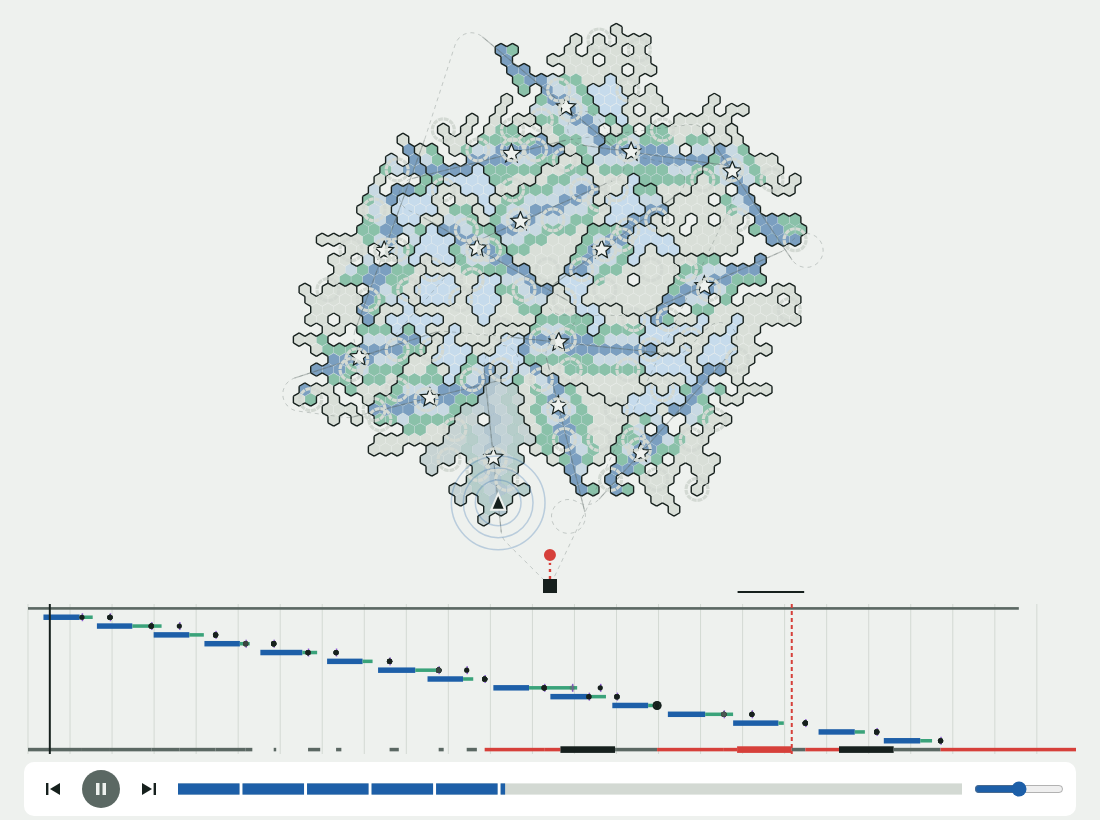
\includegraphics[width=0.82\linewidth,height=0.38\textheight,keepaspectratio]{../../../uav-l2/docs/figures/chord-anim-k16-s1-mission-frame.png}
\caption{Một nhiệm vụ trên bản đồ 15 cụm (92 critical cell), chụp
từ trang replay của mô phỏng.}
\end{figure}

\section{Đặt vấn đề và tính cấp thiết}

\subsection{Bối cảnh}

Đô thị ngày nay có mật độ camera rất cao, nhưng chúng thuộc nhiều chủ sở
hữu và phục vụ nhiều mục đích khác nhau: camera an ninh, chuông cửa, máy
bán hàng tự động, camera hành trình. Năng lực tính toán, bộ nhớ và đường
truyền của từng thiết bị rất khác nhau. Điểm chung là chúng ghi hình
liên tục và ghi đè dữ liệu cũ sau vài ngày. Khi cần tìm một người hay
một phương tiện, dữ liệu có thể đã nằm sẵn trong mạng; cái còn thiếu là
một mô tả cô đọng về đối tượng, được đặt vào từng node trước khi bằng
chứng bị ghi đè. UAV là phương tiện tự nhiên để mang một khối dữ liệu
như vậy tới một vùng rộng trong thời gian ngắn, nhất là ở nơi không có
hạ tầng mạng.

\subsection{Vấn đề cụ thể và khó khăn kỹ thuật}

Bài toán là giao một tập Q gói (khoảng 400 KB) tới mọi \textbf{critical
cell}, tức các cell có node đủ mạnh để đối sánh, từ một UAV cánh bằng
bay một lượt, sao cho thời gian hoàn thành nhiệm vụ $T^\star$ nhỏ nhất. Có bốn
khó khăn.

\begin{itemize}
\tightlist
\item
  \textbf{Kênh A2G với radio IEEE 802.15.4.} Tầm phát hiệu quả chỉ từ
  khoảng 100 m tới 1 km tuỳ môi trường (Hình 2). Fading thay đổi theo
  từng gói, nên node càng xa đường bay càng mất nhiều gói.
\item
  \textbf{Động học của UAV cánh bằng.} UAV không hover được, phải giữ
  tốc độ trên ngưỡng thất tốc và có bán kính quay tối thiểu khoảng 64 m
  ở 25 m/s. Vì vậy mỗi cụm chỉ nên được bay qua một lần.
\item
  \textbf{Liên kết đất--đất (G2G).} Liên kết này yếu hơn A2G nhiều do có
  nhiều đường NLoS và thông lượng thấp. Khi nhiều cell trao đổi cùng
  lúc, chúng tranh chấp kênh với nhau.
\item
  \textbf{Miền triển khai không lồi.} Có hồ, sông, khu cấm bay, và các
  cụm có hình dạng bất kỳ.
\end{itemize}

\begin{figure}[htbp]
\centering
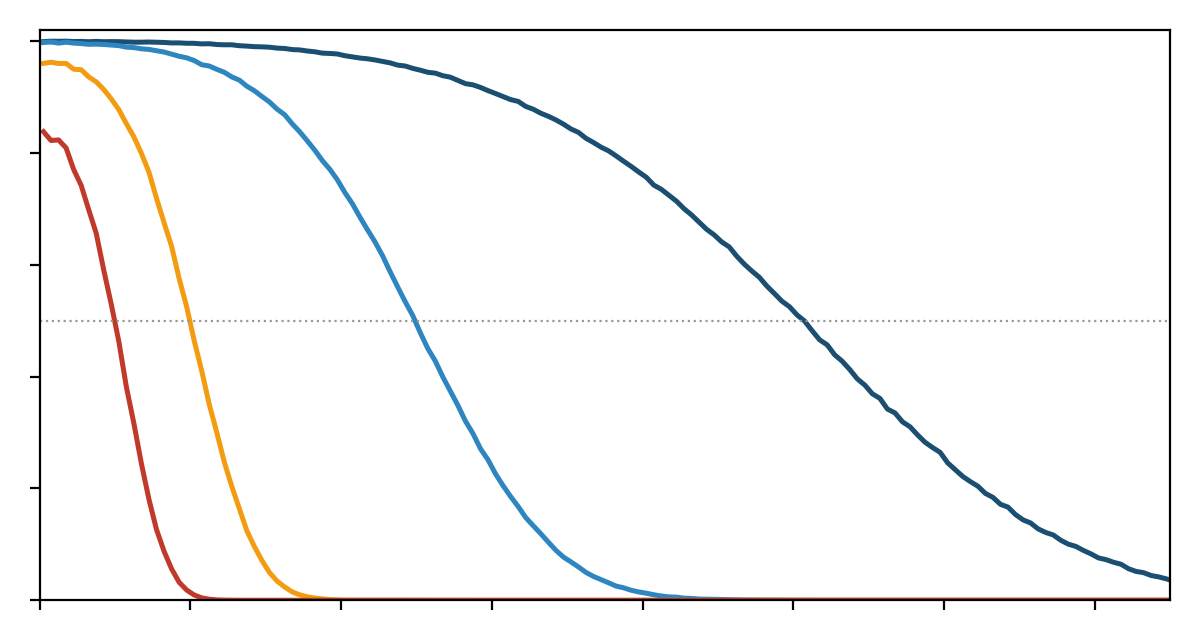
\includegraphics[width=0.82\linewidth,height=0.38\textheight,keepaspectratio]{../../../uav-l2/docs/figures/a2g-env-p-of-r-4modes.png}
\caption{Xác suất nhận gói theo khoảng cách ngang tới UAV, độ cao
100 m, ở bốn mức môi trường ($R_{50}$ ≈ 1 km, 500 m, 200 m, 100 m).}
\end{figure}

\subsection{Khoảng trống của các cách hiện có}

Các giao thức phổ tán trong WSN như Deluge và Trickle tìm dữ liệu thiếu
lúc chạy bằng quảng bá và yêu cầu. Cách này tốn nhiều frame, buộc radio
phải luôn nghe, và không biết node nào thực sự cần dữ liệu. Cách dùng
fountain code không hợp tác buộc UAV phải bay vòng hoặc giảm tốc ở từng
critical cell; khi kênh xấu, tour trở nên rất dài. Phần lớn nghiên cứu
UAV--WSN lại xét chiều thu dữ liệu từ node lên UAV, hoặc giả định UAV
hover được. Chúng tôi chưa thấy nghiên cứu nào xét việc phân phối dữ
liệu xuống bằng UAV cánh bằng, có lập kế hoạch phối hợp với mạng mặt
đất. Mục 3 trình bày chi tiết.

\subsection{Nhận xét then chốt}

Trong bài toán này, việc \textbf{gói nào rơi xuống đâu là đoán trước
được}. Đường bay và chỉ số gói đã biết trước, nên trạm gốc tính được
trước khi cất cánh cell nào sẽ nghe được đoạn dữ liệu nào. Nếu pha 0 đã
tổ chức sẵn lưới cell, cặp gateway và lịch kênh, trạm gốc có thể giao
cho từng cell một vai trò và một đoạn dữ liệu cụ thể. Khi đó phân phối
dưới mặt đất trở thành \textbf{thực thi một kế hoạch} thay vì khám phá.
Vì vậy quỹ đạo và phân phối mặt đất phải được thiết kế cùng nhau: lượt
bay quyết định SPINE nằm ở đâu và River dài bao nhiêu, còn River quyết
định critical cell nào cần UAV bay gần.

\subsection{Vì sao cấp thiết}

Bằng chứng trong camera bị ghi đè sau vài ngày, nên thời gian hoàn thành
nhiệm vụ quyết định việc có tìm được mục tiêu hay không. Cách tiếp cận
đưa truy vấn xuống còn giải quyết được vấn đề quyền riêng tư: chỉ có
điểm số rời khỏi thiết bị, dữ liệu thô không ra ngoài. Ở các vùng không
có hạ tầng như rừng, khu bảo tồn hay vùng thiên tai, đây gần như là cách
duy nhất để khai thác các camera sẵn có trong thời gian ngắn.

\section{Tổng quan nghiên cứu}

\textbf{Phổ tán dữ liệu trong WSN.}

\begin{itemize}
\tightlist
\item
  Deluge (Hui \& Culler, 2004) và MNP phát lại mã hoặc dữ liệu lớn bằng
  cơ chế quảng bá, yêu cầu theo page.
\item
  Trickle (Levis 2004, RFC 6206) điều tiết tần suất quảng bá để tiết
  kiệm năng lượng.
\item
  Đặc điểm chung: không có kế hoạch, mọi node đều phải nhận đủ, và nút
  thắt là năng lượng nghe kênh.
\end{itemize}

\textbf{Mã hoá.}

\begin{itemize}
\tightlist
\item
  Fountain code (LT, Raptor) bỏ được yêu cầu nhận đúng từng gói, nên hợp
  với kênh quảng bá có mất gói.
\item
  Network coding được dùng để tăng hiệu quả phổ tán.
\item
  Chúng tôi dùng fountain code làm baseline mạnh nhất cho trường hợp
  không hợp tác.
\end{itemize}

\textbf{UAV multicast và phân phối dữ liệu bằng UAV.}

\begin{itemize}
\tightlist
\item
  UAV làm trạm phát hoặc trạm chuyển tiếp đã được nghiên cứu rộng, phần
  lớn xét tối ưu công suất và quỹ đạo cho thông lượng.
\item
  Hướng data ferrying và DTN (message ferrying, Zhao 2004) dùng phương
  tiện di động để mang dữ liệu giữa các vùng mất kết nối.
\item
  Điểm khác ở đây: UAV phát một lần, còn mạng mặt đất hoàn tất việc phân
  phối.
\end{itemize}

\textbf{Lập quỹ đạo UAV.}

\begin{itemize}
\tightlist
\item
  Bài toán thăm các vùng tròn quanh mục tiêu với ràng buộc Dubins là
  DTSP-N, một bài toán NP-khó. Đã có nhiều thuật toán xấp xỉ.
\item
  CHORD và LM-Tour kế thừa hướng này. Khác biệt là chúng tối ưu cho thời
  gian hoàn thành ở mặt đất, không chỉ cho độ dài đường bay.
\end{itemize}

\textbf{Kênh A2G.}

\begin{itemize}
\tightlist
\item
  Mô hình xác suất LoS theo góc ngẩng (Al-Hourani 2014).
\item
  Suy hao hai đoạn và fading Rician/Nakagami theo đo đạc ở độ cao thấp
  (Qiu 2017) là cơ sở cho bốn mức môi trường dùng trong mô phỏng.
\end{itemize}

\textbf{Tổ chức mạng và lập lịch.}

\begin{itemize}
\tightlist
\item
  Phân cụm phân cấp (LEACH, HEED) và lưới địa lý (GAF) là nền của việc
  chia mạng thành cell.
\item
  Lập lịch theo khe và kênh (TSCH, 6TiSCH theo RFC 9030) cùng tô màu
  kênh là nền cho lịch các cặp gateway.
\item
  PECEE (elastic clustering) là nguồn gốc trực tiếp của lưới cell trong
  đề tài.
\end{itemize}

\textbf{Tìm kiếm tại node biên (lớp 1).}

\begin{itemize}
\tightlist
\item
  Re-ID trong kịch bản mở (open-world, ví dụ trên Market-1501) cho điểm
  vận hành để đánh đổi giữa bỏ sót và báo nhầm.
\item
  Đề tài không giải bài toán nhận dạng, chỉ dùng mô hình điểm khớp trích
  từ các công bố này (\texttt{research\_notes/l1-*}).
\end{itemize}

\textbf{Học máy cho lập quỹ đạo.}

\begin{itemize}
\tightlist
\item
  Hướng dùng mô hình dự đoán (surrogate) học từ mô phỏng để thay thế
  phép đánh giá tốn kém trong vòng lặp tối ưu. LM-Tour thuộc hướng này.
  \textbf{{[}cần khảo sát thêm{]}}
\end{itemize}

Bảng dưới định vị đề tài so với các nhóm trên (bản nháp, cần rà lại sau
khi khảo sát đầy đủ).

\begin{longtable}[]{@{}llllll@{}}
\toprule\noalign{}
Nhóm & Biết trước nội dung và đích & Đơn vị kế hoạch là cell & UAV cánh
bằng một lượt & Hợp tác mặt đất có lịch & Đánh giá packet-level \\
\midrule\noalign{}
\endhead
\bottomrule\noalign{}
\endlastfoot
Deluge, Trickle & không & không & --- & không & có \\
Fountain code từ UAV & một phần & không & thường hover & không & ít \\
UAV thu dữ liệu WSN & --- & đôi khi & thường hover & không & ít \\
DTSP-N & có (vị trí) & không & có & không & không \\
\textbf{SigDrop} & \textbf{có} & \textbf{có} & \textbf{có} & \textbf{có}
& \textbf{có (ns-3)} \\
\end{longtable}

\section{Kết quả bước đầu}

\subsection{Bài ICC 2027 và các đóng góp chính}

Bài SigDrop gửi IEEE ICC 2027 (bản v5.3, LaTeX ở \texttt{paper/icc-v5/})
có bốn đóng góp.

\textbf{Kiến trúc phát truy vấn một lượt, lập kế hoạch trước.}

\begin{itemize}
\tightlist
\item
  Mạng được tổ chức sẵn thành lưới cell lục giác. Mỗi cell có một CL,
  mỗi cặp cell kề có một cặp gateway, và các cặp gateway dùng lịch kênh
  7 màu.
\item
  Trước khi cất cánh, trạm gốc tính được cell nào nghe được đoạn gói
  nào, nhờ biết trước đường bay và nhịp phát. Từ đó nó giao cho từng
  cell một vai trò.
\item
  UAV cánh bằng chỉ bay qua mỗi cụm một lần. Phân phối dưới mặt đất diễn
  ra theo kế hoạch, không cần khám phá nội dung lúc chạy.
\end{itemize}

\textbf{Cơ chế River (lớp 3).}

\begin{itemize}
\tightlist
\item
  \textbf{SPINE:} các cell nằm dưới đường bay. Mỗi SPINE cell được giao
  một đoạn gói Seg, phát theo thứ tự UAV bay qua.
\item
  \textbf{Bank:} dựng theo đường vuông góc với SPINE, nhận dữ liệu từ
  SPINE.
\item
  \textbf{Ring:} các cell quanh mỗi critical cell, lấy dữ liệu từ Bank
  theo các đường cell đã lập sẵn. Kích thước Ring tuỳ lượng dữ liệu
  critical cell còn thiếu.
\item
  \textbf{Sửa lỗi} gồm ba bước: SPINE cell lấy bù đoạn của mình từ cell
  kề; critical cell hỏi lại khi đứng yên quá lâu; và takeover khi đường
  bay thật lệch khỏi kế hoạch.
\end{itemize}

\textbf{Hai thiết kế quỹ đạo (lớp 2).}

\begin{itemize}
\tightlist
\item
  \textbf{CHORD:} mỗi cụm một đường thẳng qua CH, theo hướng có đoạn nằm
  trong cụm dài nhất. Đường được cắt vừa đủ dữ liệu, uốn nhẹ về các
  critical cell gần đó, và nối các cụm bằng đường Dubins.
\item
  \textbf{LM-Tour:} dựng tour DTSP-N qua đĩa bán kính ξ quanh các CH.
  Sau đó uốn dần tour về các landmark có trọng số cao, tới khi lợi ích
  bão hoà. Lợi ích được đánh giá bằng một bộ dự đoán thời gian River học
  từ chính dữ liệu ns-3.
\end{itemize}

\textbf{Mô hình nhiệm vụ đầu--cuối.}

\begin{itemize}
\tightlist
\item
  \textbf{Lớp 1:} mỗi node có một kho ảnh mang điểm khớp ngẫu nhiên. Ảnh
  tham chiếu có trọng số độ quan trọng do trạm gốc chấm. Critical cell
  đối sánh xong thì gửi điểm cao nhất về trạm gốc qua LoRa.
\item
  \textbf{Pha 2:} đội UAV thứ hai thăm các cell theo điểm nghi vấn.
\item
  \textbf{$T^\star$:} thời điểm xác minh xong cell có điểm cao nhất.
\end{itemize}

\begin{figure}[htbp]
\centering
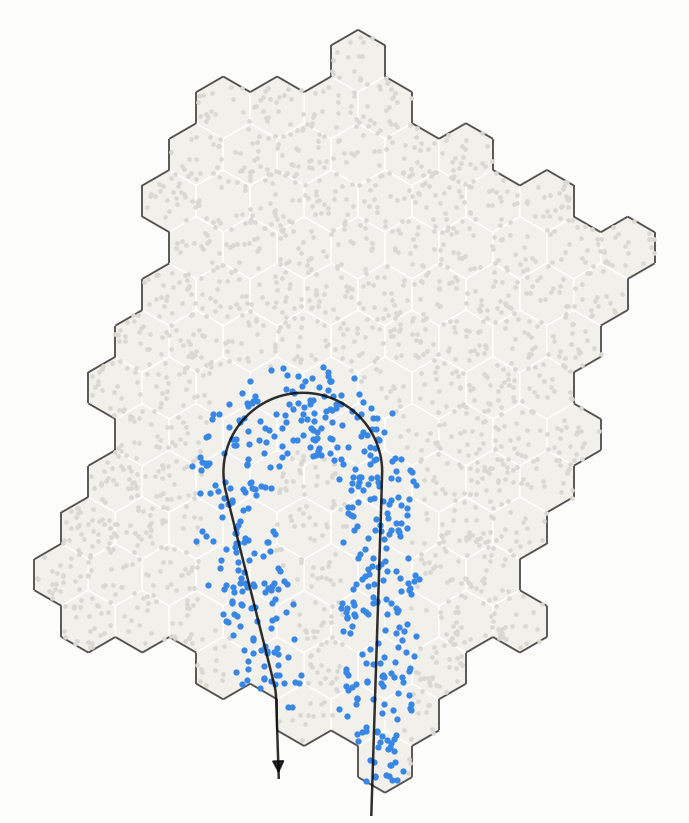
\includegraphics[width=0.82\linewidth,height=0.38\textheight,keepaspectratio]{../../../uav-coop2/docs/figures/concept-river.png}
\caption{River trên một cụm: các cell đậm dưới đường bay là SPINE,
nhận trực tiếp phần lớn dữ liệu; các cell nhạt dần ra hai bên là Bank và
vùng phục vụ.}
\end{figure}

\begin{figure}[htbp]
\centering
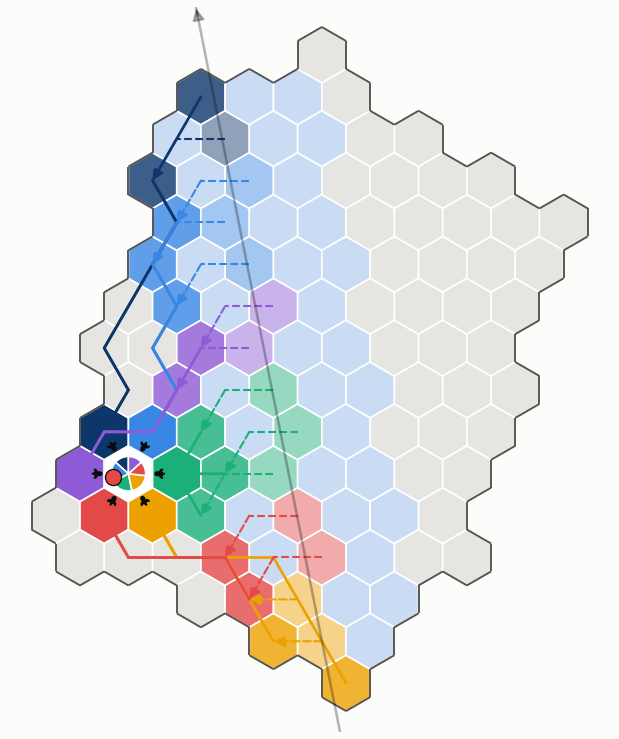
\includegraphics[width=0.82\linewidth,height=0.38\textheight,keepaspectratio]{../../../uav-coop2/docs/figures/concept-circle.png}
\caption{Ring: các cell quanh một critical cell, mỗi cell đảm nhận
một phần dữ liệu còn thiếu, lấy từ Bank theo đường cell đã lập sẵn.}
\end{figure}

\subsection{Thuật toán đã có}

Bài ICC trình bày bốn thuật toán dạng mã giả:

\begin{itemize}
\tightlist
\item
  \textbf{Lập bảng Seg tại trạm gốc:} mỗi SPINE cell được phục vụ đoạn
  gói nào.
\item
  \textbf{Thiết lập River:} chọn Bank theo pháp tuyến của SPINE, chọn
  critical cell và Ring.
\item
  \textbf{CHORD:} chọn hướng, cắt, uốn và nối các cụm.
\item
  \textbf{LM-Tour:} DTSP-N qua các CH rồi uốn về landmark, với tham số
  ξ.
\end{itemize}

Sau bài ICC, ba phần được bổ sung:

\begin{itemize}
\tightlist
\item
  \textbf{Takeover:} sau bước sửa từ cell kề, SPINE cell còn thiếu gói
  sẽ hỏi lan trong 3 hop cell bằng frame điều khiển; cell giữ gói trả
  lời bằng dữ liệu.
\item
  \textbf{Biến thể takeover theo tọa độ trong header:} cell dưới đường
  bay thật tự báo cho SPINE cell bị ảnh hưởng.
\item
  \textbf{Bộ dự đoán thời gian River dạng cây,} dùng trong LM-Tour.
\end{itemize}

\subsection{Đo lường}

Năm nhóm chỉ số:

\begin{itemize}
\tightlist
\item
  \textbf{$T^\star$:} chỉ số chính. Lấy trung bình trên 100 lượt bốc lớp 1 ghép
  cặp mỗi seed, để tách nhiễu của lớp 1 khỏi khác biệt giữa các phương
  án.
\item
  \textbf{Thời điểm sẵn sàng:} với mỗi cụm, lúc critical cell cuối cùng
  nhận đủ, tính từ khi UAV rời cụm; sau đó lấy trung bình qua các cụm.
  Kèm theo là tỉ lệ critical cell nhận đủ trước giới hạn 900 s.
\item
  \textbf{Số frame phát dưới mặt đất:} gồm dữ liệu, yêu cầu, quảng bá,
  ACK và phát lại.
\item
  \textbf{Năng lượng radio:} tính từ thời gian mỗi node ở các trạng thái
  PHY (phát, nhận, nghe, tắt). Có hai chip (CC2420, EFR32MG21) và hai
  chế độ: luôn nghe, và ngủ theo lịch sau frame cuối của mình. Báo cáo
  cả tổng và node nóng nhất.
\item
  \textbf{Năng lượng và quãng bay của UAV:} theo mô hình Zeng--Zhang cho
  cánh bằng.
\end{itemize}

\subsection{Thiết lập giả lập}

\textbf{Mô phỏng.}

\begin{itemize}
\tightlist
\item
  ns-3.46 với lớp lr-wpan đầy đủ: PHY 802.15.4 2,4 GHz, MAC CSMA/CA
  không khe có ACK, mỗi node một thiết bị.
\item
  Lịch kênh 7 màu cho các cặp gateway, theo lưới PECEE.
\end{itemize}

\textbf{Kênh.}

\begin{itemize}
\tightlist
\item
  \textbf{A2G:} suy hao hai đoạn neo tại độ cao bay, fading Nakagami (m
  = 1,8) bốc lại mỗi gói.
\item
  Bốn mức môi trường thêm suy hao 0 / 9,0 / 19,8 / 25,7 dB. Bán kính 50
  \% tương ứng khoảng 1 015 / 498 / 199 / 99 m (Hình 2).
\item
  \textbf{G2G:} suy hao log-distance, kèm shadowing và fading gắn với
  từng cặp node.
\end{itemize}

\textbf{Kịch bản.}

\begin{itemize}
\tightlist
\item
  Bản đồ là miền không lồi có hồ, chia thành 8, 12 và 15 cụm; mỗi cụm
  tối đa 80 cell lục giác R = 100 m.
\item
  Truy vấn khoảng 400 KB, Q ≈ 4 041 gói, phát 10 ms một gói.
\item
  UAV bay theo hồ sơ tốc độ có giới hạn góc nghiêng 45°.
\end{itemize}

\textbf{Cách chạy.}

\begin{itemize}
\tightlist
\item
  Lượt bay của UAV được mô phỏng trước, ghi lại node nào nhận gói nào.
\item
  Sau đó, phần phân phối dưới mặt đất của từng cụm chạy riêng trên kết
  quả đó.
\item
  Phương án nhận cùng lượt bay, cùng kênh và cùng seed để so sánh ghép
  cặp.
\item
  Sai lệch quỹ đạo do gió được tạo bằng nhiễu trắng làm mượt, lệch ngang
  thực tế lên tới vài trăm mét.
\end{itemize}

\subsection{Kết quả chính}

\begin{longtable}[]{@{}lll@{}}
\toprule\noalign{}
Thí nghiệm & Thiết lập & Kết quả \\
\midrule\noalign{}
\endhead
\bottomrule\noalign{}
\endlastfoot
C4 & 3 bản đồ × 4 kênh & LM-Tour + River nhanh nhất trong các phương án
thực tế: nhanh hơn CHORD + River 1--11 \%, DTSP-N + River 10--26 \%, FC
+ DTSP-N 10--72 \%. Ở r200/r100, các phương án có River nhanh hơn FC +
DTSP-N 49--72 \% \\
LMT, T3S & 812 critical cell & Bộ dự đoán thời gian River dạng cây sai
số 26,2 s, so với 45,9 s của công thức tuyến tính \\
DLG & cùng lượt CHORD, k8, r100, 5 seed & So với Deluge: sẵn sàng 117 so
với 149--156 s; ít frame hơn 1,9--2,5 lần; ít năng lượng radio hơn
6,5--8,8 lần khi ngủ theo lịch, nhưng ngang nhau khi luôn nghe; $T^\star$ nhanh
hơn 36--43 s, thắng 5/5 seed \\
WND, TKO & gió σ = 50/100 m, 3 seed & Ở σ = 100 m (lệch ngang tới 346
m), không có takeover chỉ 106/135 cell xong, $T^\star$ +294 s. Takeover tuần
tự: 135/135 cell, sẵn sàng 112--118 s, $T^\star$ bằng danh nghĩa trong phạm vi
nhiễu (−22 ± 184 s) \\
\end{longtable}

\begin{figure}[htbp]
\centering
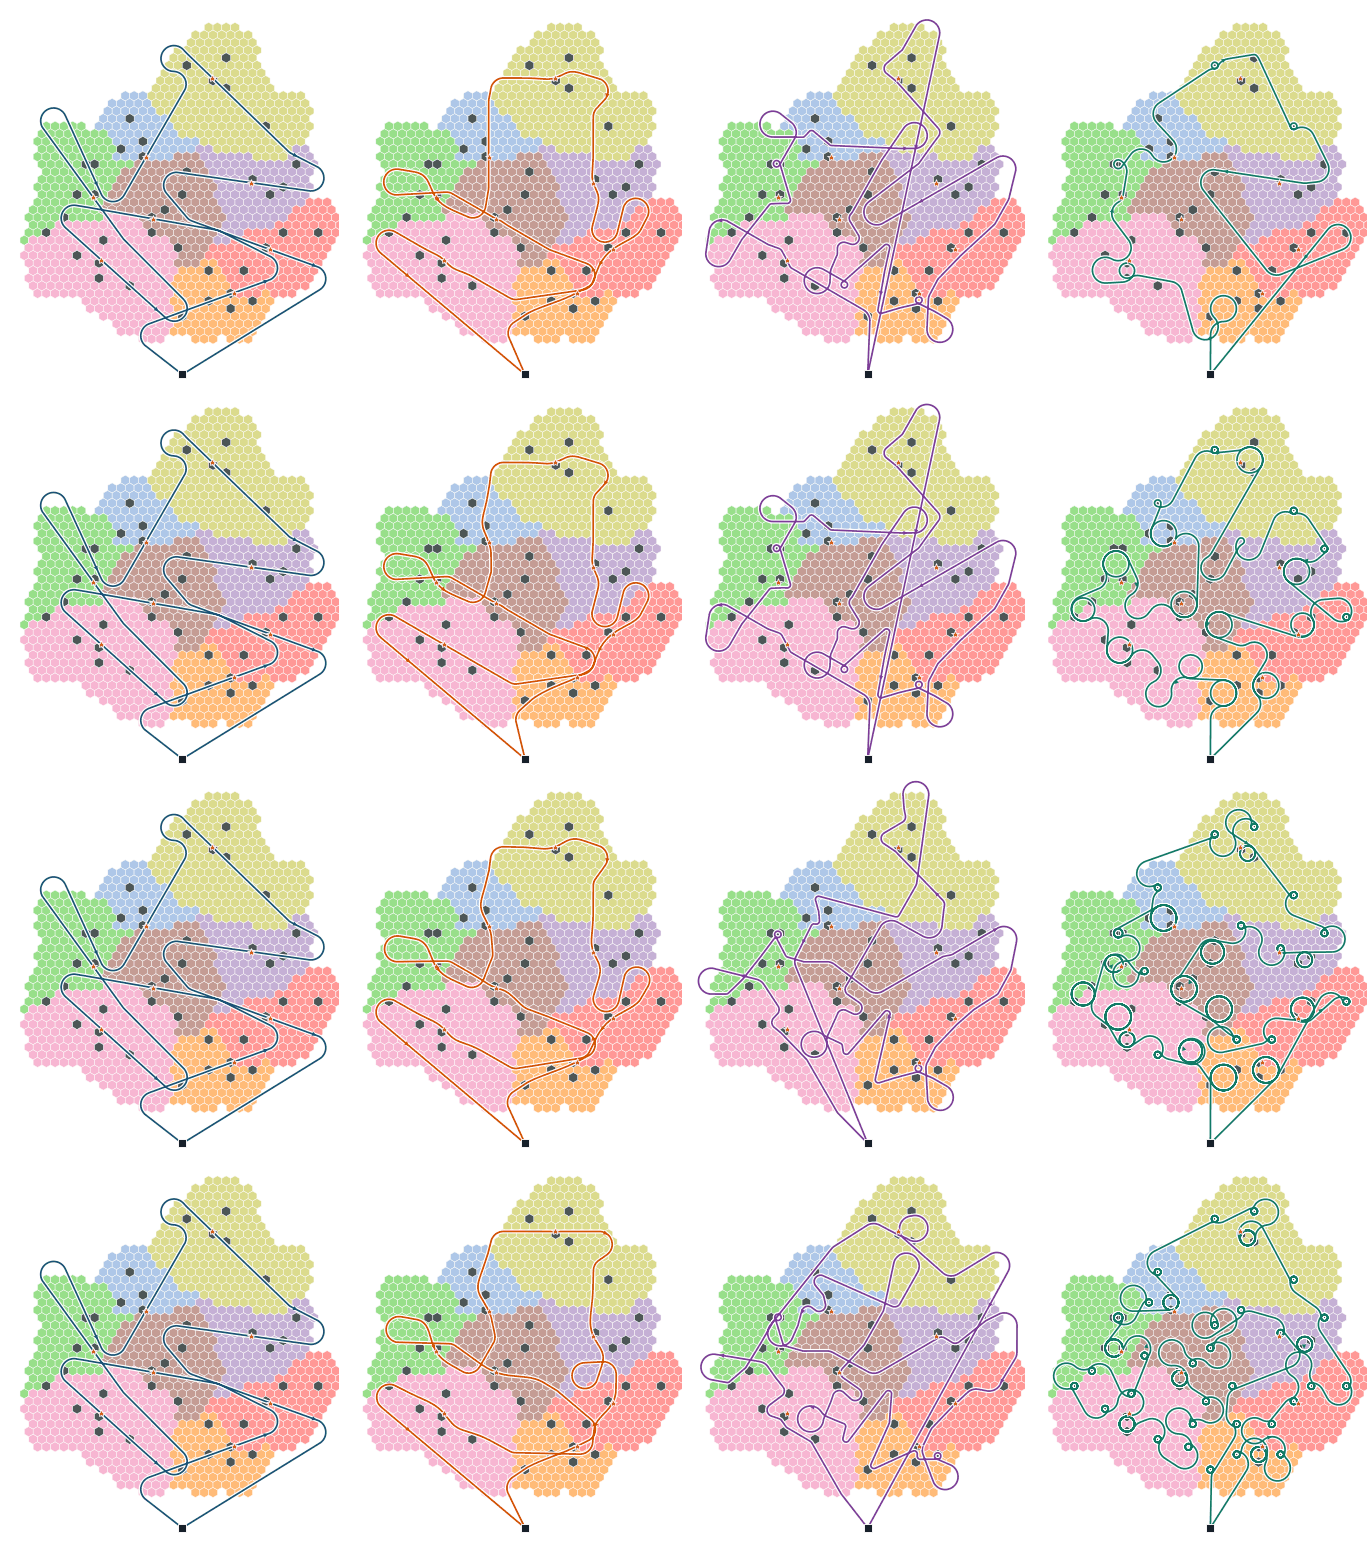
\includegraphics[width=0.82\linewidth,height=0.38\textheight,keepaspectratio]{../../../uav-l2/docs/figures/c4-phase1/c4-phase1-k8-s1-grid.png}
\caption{Đường bay pha 1 trên bản đồ 8 cụm. Hàng là mức kênh (open,
r500, r200, r100); cột là phương án (CHORD + River, LM-Tour + River,
DTSP-N + River, FC + DTSP-N). Khi kênh xấu đi, FC + DTSP-N phải bay vòng
ngày càng nhiều quanh các critical cell.}
\end{figure}

\begin{figure}[htbp]
\centering
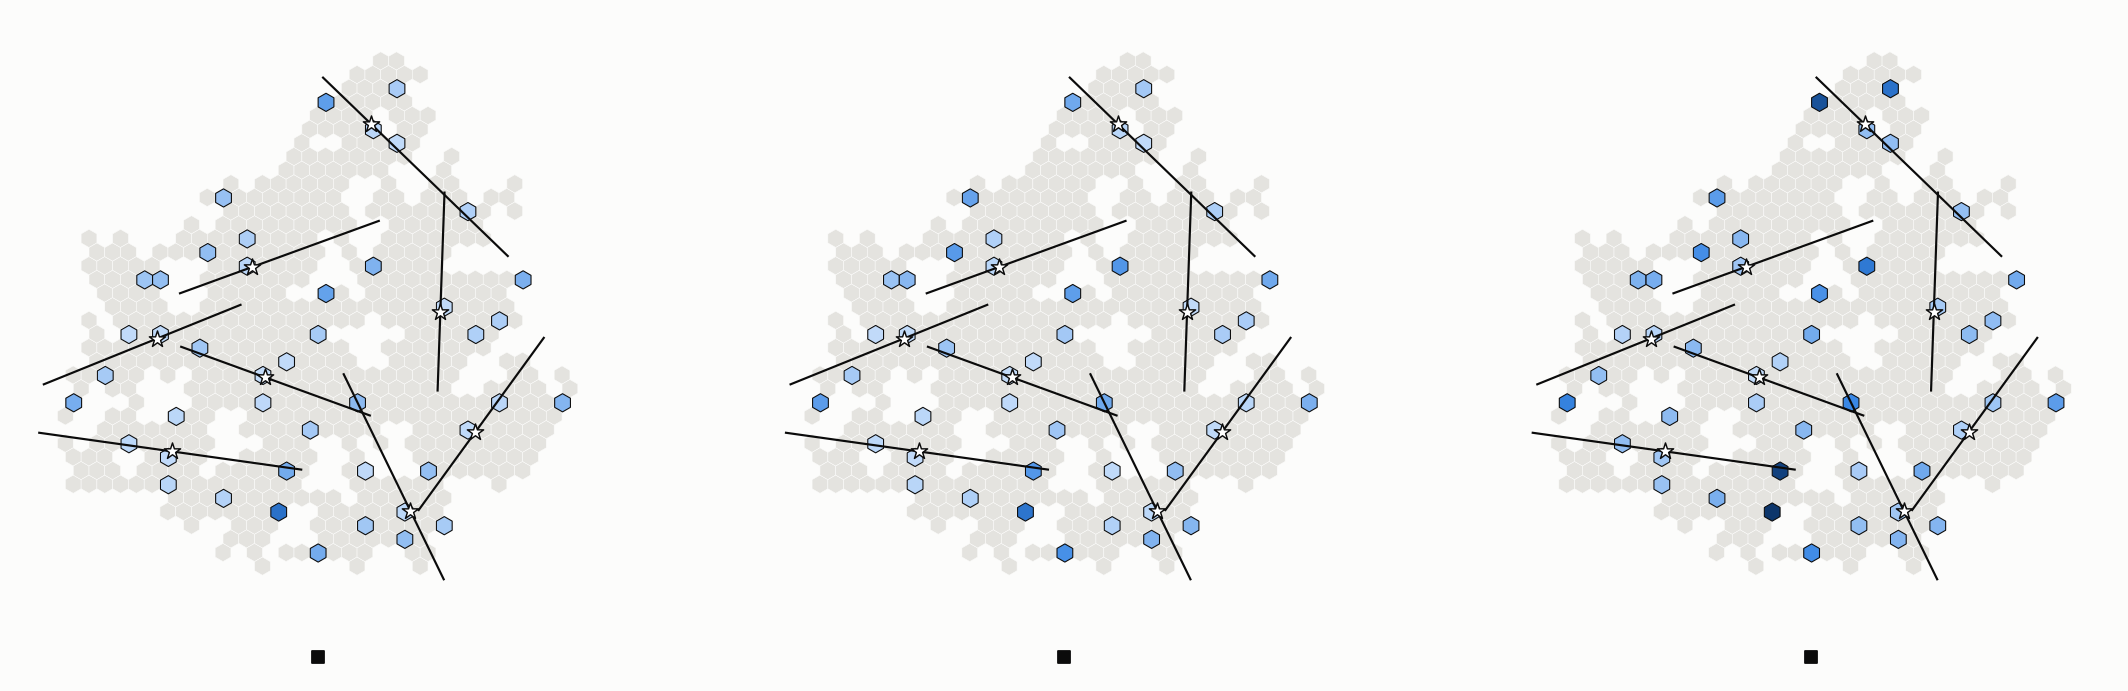
\includegraphics[width=0.82\linewidth,height=0.38\textheight,keepaspectratio]{../../../uav-l2/docs/figures/cmp-k8-s1-layer3-river-direct-trickle.png}
\caption{Ba cách phân phối dưới mặt đất trên cùng một lượt bay:
River, kéo trực tiếp và Trickle.}
\end{figure}

\subsection{Hạn chế về logic, tính thực tế và độ chắc của lập
luận}

Mục này chỉ nêu các điểm yếu về lập luận và giả định. Những phần chỉ
thiếu thời gian chạy thì không nêu ở đây.

\textbf{Kế hoạch và mô phỏng dùng cùng một mô hình kênh.}

\begin{itemize}
\tightlist
\item
  Trạm gốc lập kế hoạch (SPINE, độ rộng River, Seg) dựa trên mô hình xác
  suất nhận gói, và mô phỏng cũng chạy đúng mô hình đó. Kết quả vì vậy
  đánh giá quá cao độ chính xác của kế hoạch.
\item
  Ngoài đời, kênh thật lệch khỏi mô hình lập kế hoạch. Sai lệch này chưa
  được đo riêng; thử nghiệm gió mới chỉ kiểm phần sai lệch về quỹ đạo.
\end{itemize}

\textbf{Các cụm được mô phỏng tách rời, và phân phối mặt đất chỉ bắt đầu
sau khi UAV rời cụm.}

\begin{itemize}
\tightlist
\item
  Không có nhiễu giữa các cụm, không có hợp tác xuyên cụm, và gói UAV
  phát không va chạm với lưu lượng dưới đất.
\item
  Trong thực tế, cụm vừa được bay qua sẽ trao đổi dữ liệu đúng lúc UAV
  phát cho cụm kế bên.
\item
  Mốc "sẵn sàng tính từ lúc UAV rời cụm" cũng bỏ qua khả năng bắt đầu
  phân phối sớm hơn.
\end{itemize}

\textbf{Pha 0 được coi là miễn phí và cố định.}

\begin{itemize}
\tightlist
\item
  Chi phí bầu CL, chọn gateway, phát bảng định tuyến và đồng bộ lịch
  kênh không được tính.
\item
  Mạng được coi là đứng yên, không node hỏng, mọi thiết bị đều hợp tác.
  Giả định cuối mâu thuẫn với chính bối cảnh thiết bị thuộc nhiều chủ sở
  hữu.
\item
  Toàn bộ node được coi là thức để nghe UAV trong lượt bay. Điều này cần
  một cơ chế đánh thức đúng giờ, chưa được mô tả.
\end{itemize}

\textbf{Lớp 1 và pha 2 chỉ là mô hình trừu tượng.}

\begin{itemize}
\tightlist
\item
  Phân bố điểm khớp và trọng số manh mối là giả định; thời gian đối sánh
  lấy từ số liệu công bố.
\item
  Chỉ có một mục tiêu, và điểm nghi vấn thật luôn nằm ở một critical
  cell.
\item
  Đội 2 được mô hình bằng thời gian bay, hover và tải tệp cố định; trễ
  LoRa là một hằng số.
\item
  $T^\star$ vì vậy nhạy với các giả định này: chênh lệch ±100 s giữa các seed
  chủ yếu đến từ lớp 1, không phải từ mạng.
\end{itemize}

\textbf{Mô hình kênh lạc quan ở chỗ fading.}

\begin{itemize}
\tightlist
\item
  Fading được giữ không đổi trong một gói. Nhưng ở tốc độ bay, thời gian
  kết hợp của kênh (khoảng 1 ms) ngắn hơn thời gian chiếm sóng của gói
  (4,3 ms).
\item
  Kết quả mất gói A2G vì vậy lạc quan. Giới hạn này đã được ghi nhận từ
  thí nghiệm A2G-RUN nhưng chưa được hiệu chỉnh.
\end{itemize}

\textbf{Lợi thế năng lượng của River phụ thuộc giả định ngủ.}

\begin{itemize}
\tightlist
\item
  Khi mọi node luôn nghe, năng lượng radio của River và Deluge ngang
  nhau.
\item
  Mức lợi 6,5--8,8 lần chỉ xuất hiện khi giả định node ngủ ngay sau
  frame cuối của mình. Con số này là một chặn tính sau khi chạy, không
  phải cơ chế ngủ được mô phỏng, nên cần phát biểu thận trọng.
\end{itemize}

\textbf{So sánh giữa các phương án chưa hoàn toàn cùng điều kiện.}

\begin{itemize}
\tightlist
\item
  FC được mô hình với fountain code lý tưởng (ε = 5 \%).
\item
  CHORD và LM-Tour dùng bộ manh mối mã fountain ở mức mô hình nhiệm vụ,
  nhưng River trong ns-3 vẫn vận chuyển gói gốc.
\item
  Một số ô của LM-Tour là ước lượng mức mô hình (thời gian River lấy từ
  bộ dự đoán), không phải số chạy ns-3.
\end{itemize}

\textbf{Bộ dự đoán được học và kiểm tra trên cùng các bản đồ.}

\begin{itemize}
\tightlist
\item
  Chưa có kiểm định trên bản đồ chưa thấy, nên lợi thế của LM-Tour có
  thể một phần đến từ việc khớp quá mức.
\item
  Điều kiện "uốn tới khi lợi ích bão hoà" là heuristic, chưa có bảo đảm.
\end{itemize}

\textbf{Một số lựa chọn thiết kế thuận lợi cho đề xuất.}

\begin{itemize}
\tightlist
\item
  CH được chọn là node mạnh nhất, cách biên ít nhất 300 m. Thử với CH ở
  vị trí ngẫu nhiên cho thấy kết quả kém đi rõ.
\item
  Critical cell do trạm gốc chọn theo năng lực, nhưng chưa có lý do lý
  thuyết cho số lượng và vị trí của chúng.
\end{itemize}

\textbf{Lập luận "lập kế hoạch tốt hơn khám phá" mới dựa trên thực
nghiệm.}

\begin{itemize}
\tightlist
\item
  Chưa có định lý về tính đầy đủ, cận dưới hay độ lợi theo chất lượng
  kênh. Các con số đến từ một số ít bản đồ và một cách cấu hình Deluge.
\item
  Nếu Deluge được tinh chỉnh tốt hơn (Deluge-lite), khoảng cách về thời
  gian có thể thu hẹp. Khi đó luận điểm phải dựa vào số frame và việc
  không cần khám phá, thay vì thời gian.
\end{itemize}

\section{Mục tiêu và câu hỏi nghiên cứu}

\subsection{Mục tiêu tổng quát}

Xây dựng một lời giải đầy đủ cho cả ba pha: tổ chức mạng, phát truy vấn
và xác minh. Lời giải phải có bảo đảm hình thức về tính đúng (mọi
critical cell nhận đủ dữ liệu) và về thời gian hoàn thành, bền vững
trước sai lệch thực tế, và được kiểm chứng trên phần cứng 802.15.4.

\subsection{Mục tiêu cụ thể}

\begin{itemize}
\tightlist
\item
  \textbf{MT0 (pha 0):} thiết kế và đo chi phí dựng, duy trì lưới cell
  (CL, gateway, định tuyến, lịch kênh) bằng frame thật.
\item
  \textbf{MT1 (cả ba pha):} mô hình hoá bài toán đầu--cuối, chứng minh
  độ khó, tìm cận dưới của $T^\star$ và các định lý bảo đảm.
\item
  \textbf{MT2 (pha 1, lớp 3):} hoàn thiện River, takeover và biến thể
  dùng fountain code.
\item
  \textbf{MT3 (pha 1, lớp 2):} lập quỹ đạo có bộ dự đoán, có bảo đảm xấp
  xỉ và khả năng tổng quát hoá, mở rộng cho nhiều UAV.
\item
  \textbf{MT4 (pha 2):} lập lịch đội xác minh theo điểm nghi vấn, có
  tính thời gian hover, tải tệp lớn và trễ kênh phản hồi LoRa; liên kết
  với mô hình lớp 1 để đánh giá xác suất tìm thấy mục tiêu.
\item
  \textbf{MT5:} đánh giá đầu--cuối ở quy mô lớn và kiểm chứng trên phần
  cứng.
\end{itemize}

\subsection{Câu hỏi nghiên cứu}

\begin{itemize}
\tightlist
\item
  \textbf{RQ0 (ND0):} dựng và duy trì lưới cell tốn bao nhiêu frame,
  thời gian và năng lượng, và chi phí đó tăng thế nào theo mật độ node?
\item
  \textbf{RQ1 (ND1):} dưới điều kiện nào River bảo đảm mọi critical cell
  nhận đủ dữ liệu; cận dưới của $T^\star$ là bao nhiêu, và lời giải cách cận đó
  bao xa?
\item
  \textbf{RQ2 (ND2):} lập kế hoạch trước có lợi hơn khám phá lúc chạy
  đến đâu, và fountain code thay đổi lợi thế đó thế nào?
\item
  \textbf{RQ3 (ND2, ND4):} lời giải còn đứng vững tới mức sai lệch đường
  bay, tỉ lệ node hỏng và độ xấu kênh nào?
\item
  \textbf{RQ4 (ND3):} bộ dự đoán giúp quỹ đạo tốt hơn bao nhiêu, và có
  dùng được trên bản đồ chưa thấy không?
\item
  \textbf{RQ5 (ND6):} thứ tự và cách xác minh ở pha 2 ảnh hưởng thế nào
  tới thời gian tìm thấy mục tiêu thật?
\item
  \textbf{RQ6 (ND5):} kết quả mô phỏng còn giữ được bao nhiêu trên phần
  cứng thật?
\end{itemize}

\subsection{Đóng góp dự kiến}

\begin{enumerate}
\def\labelenumi{\arabic{enumi}.}
\tightlist
\item
  Kiến trúc ba pha, trong đó phân phối dưới mặt đất được lập kế hoạch
  trước nhờ tổ chức lưới cell.
\item
  Giao thức River kèm takeover, tự thích ứng khi đường bay lệch khỏi kế
  hoạch.
\item
  Cách lập quỹ đạo có bộ dự đoán (LM-Tour).
\item
  Mô hình và cận dưới cho bài toán.
\item
  Bộ mô phỏng ns-3 và bộ dữ liệu công khai.
\end{enumerate}

\section{Đối tượng và phạm vi}

\subsection{Đối tượng nghiên cứu}

Đối tượng là mạng camera IoT không đồng nhất dùng radio IEEE 802.15.4,
tổ chức theo lưới cell lục giác. Pha 1 dùng UAV cánh bằng để phát truy
vấn, pha 2 dùng UAV cánh quay để xác minh. Truy vấn là một bộ ảnh tham
chiếu khoảng 400 KB, chia thành các gói 802.15.4.

\subsection{Phạm vi}

\textbf{Trong phạm vi:}

\begin{itemize}
\tightlist
\item
  pha 0 (tổ chức mạng theo lưới cell);
\item
  pha 1, gồm lớp 2 (quỹ đạo) và lớp 3 (River);
\item
  thời gian của pha 2, ở mức mô hình;
\item
  kênh A2G và G2G, MAC 802.15.4, năng lượng radio và năng lượng UAV;
\item
  miền không lồi có vật cản mềm (hồ, sông: bay qua được nhưng không có
  node).
\end{itemize}

\textbf{Ngoài phạm vi:}

\begin{itemize}
\tightlist
\item
  Thuật toán nhận dạng ảnh. Lớp 1 chỉ dùng mô hình điểm khớp đã chốt, có
  nguồn công bố.
\item
  Bảo mật và quyền sở hữu thiết bị: chỉ nêu ở phần hướng mở.
\item
  Vật cản cứng và khu cấm bay. \textbf{{[}cần chốt{]}} Có thể đưa vào
  ND4 nếu còn thời gian.
\end{itemize}

\subsection{Giả định chính}

\begin{itemize}
\tightlist
\item
  Pha 0 hoàn tất trước nhiệm vụ. Trong suốt nhiệm vụ, lưới cell, CL, cặp
  gateway, bảng định tuyến và lịch kênh không đổi, và trạm gốc biết toàn
  bộ.
\item
  Node đứng yên. UAV biết vị trí của mình nhờ GPS và có thể ghi tọa độ
  vào header của mỗi gói.
\item
  Các ảnh tham chiếu không thay thế được cho nhau, nên mỗi critical cell
  cần đủ Q gói.
\item
  Báo cáo điểm số về trạm gốc đi qua LoRa hoặc vệ tinh, với độ trễ do
  giới hạn chu kỳ phát.
\end{itemize}

\subsection{Chỉ số đánh giá}

\begin{itemize}
\tightlist
\item
  \textbf{$T^\star$} (chỉ số chính): thời gian hoàn thành nhiệm vụ. Lấy trung
  bình trên 100 lượt bốc lớp 1 ghép cặp mỗi seed.
\item
  \textbf{Thời điểm sẵn sàng}: thời điểm critical cell cuối cùng của mỗi
  cụm nhận đủ dữ liệu, tính từ khi UAV rời cụm, rồi lấy trung bình qua
  các cụm.
\item
  \textbf{Tỉ lệ critical cell nhận đủ.}
\item
  \textbf{Số frame phát dưới mặt đất.}
\item
  \textbf{Năng lượng radio}: tổng toàn mạng và node tốn nhất, tính cho
  hai chip CC2420 và EFR32.
\item
  \textbf{Năng lượng UAV}: theo mô hình có số hạng gia tốc.
\end{itemize}

\section{Nội dung và phương pháp nghiên cứu}

\subsection{Phương pháp chung}

\textbf{Công cụ.}

\begin{itemize}
\tightlist
\item
  Mô phỏng chính chạy trên ns-3.46 với lớp lr-wpan.
\item
  Mỗi chiến dịch dùng một bộ binary đã chốt, ghi sha256 trong log.
\item
  Lập quỹ đạo và mô hình lớp 1 viết bằng Python.
\item
  Mọi tham số tập trung trong \texttt{params.yaml}.
\end{itemize}

\textbf{Thống kê.}

\begin{itemize}
\tightlist
\item
  So sánh luôn ghép cặp: các phương án chạy trên cùng lượt bay, cùng
  kênh và cùng seed.
\item
  Báo cáo khoảng tin cậy 95 \% theo seed, kèm số seed mà phương án đề
  xuất thắng.
\item
  Kết luận chính cần ít nhất 5 seed; không kết luận từ một seed.
\end{itemize}

\textbf{Baseline.}

\begin{itemize}
\tightlist
\item
  Deluge/Trickle, chạy trên hai phạm vi: các cell của River và các cell
  trên đường kéo.
\item
  Kéo trực tiếp.
\item
  FC + DTSP-N.
\item
  DTSP-N + River.
\item
  CHORD.
\end{itemize}

\textbf{Tái lập.}

\begin{itemize}
\tightlist
\item
  Mỗi lần chạy có một thư mục log kèm README.
\item
  Mỗi thí nghiệm có mã riêng trong \texttt{docs/EXPERIMENTS-INDEX.md}.
\end{itemize}

\subsection{ND0. Tổ chức mạng theo lưới cell (pha 0)}

\textbf{Mục tiêu.} ND0 biến pha 0 từ một bước "tính sẵn, miễn phí" thành
một giao thức có chi phí đo được và một quy tắc thiết kế rõ ràng. Nó trả
lời RQ0.

\textbf{Hiện trạng.} Trong mô phỏng hiện tại, pha 0 được tính sẵn tại
trạm gốc:

\begin{itemize}
\tightlist
\item
  \textbf{Lưới và vai trò.} Mạng được chia thành lưới lục giác bán kính
  R ≥ 100 m, chọn theo mật độ và kích thước mạng. Mỗi cell chọn một CL
  (node có năng lực tốt nhất). Mỗi cặp cell kề có đúng một cặp gateway,
  là cặp node có liên kết tốt nhất qua cạnh chung.
\item
  \textbf{Định tuyến.} Mỗi node giữ bảng định tuyến PECEE: next hop tới
  CL của cell mình (theo ETX nhỏ nhất) và tới từng cell kề.
\item
  \textbf{Lịch kênh.} Lưu lượng trong cell dùng 7 kênh, xếp theo lưới 7
  màu, sao cho hai cell cùng kênh cách nhau ít nhất 3 bước cell. Mỗi cặp
  gateway dùng một kênh riêng trong 9 kênh còn lại, không trùng với cặp
  nào ở gần. Node gateway có radio riêng cho kênh cặp, tức là một giả
  định đa radio.
\item
  \textbf{Cụm và vai trò của trạm gốc.} Mỗi cụm có tối đa 80 cell. Trạm
  gốc chọn CH và các critical cell, rồi phát kế hoạch xuống trước mỗi
  nhiệm vụ.
\end{itemize}

\begin{figure}[htbp]
\centering
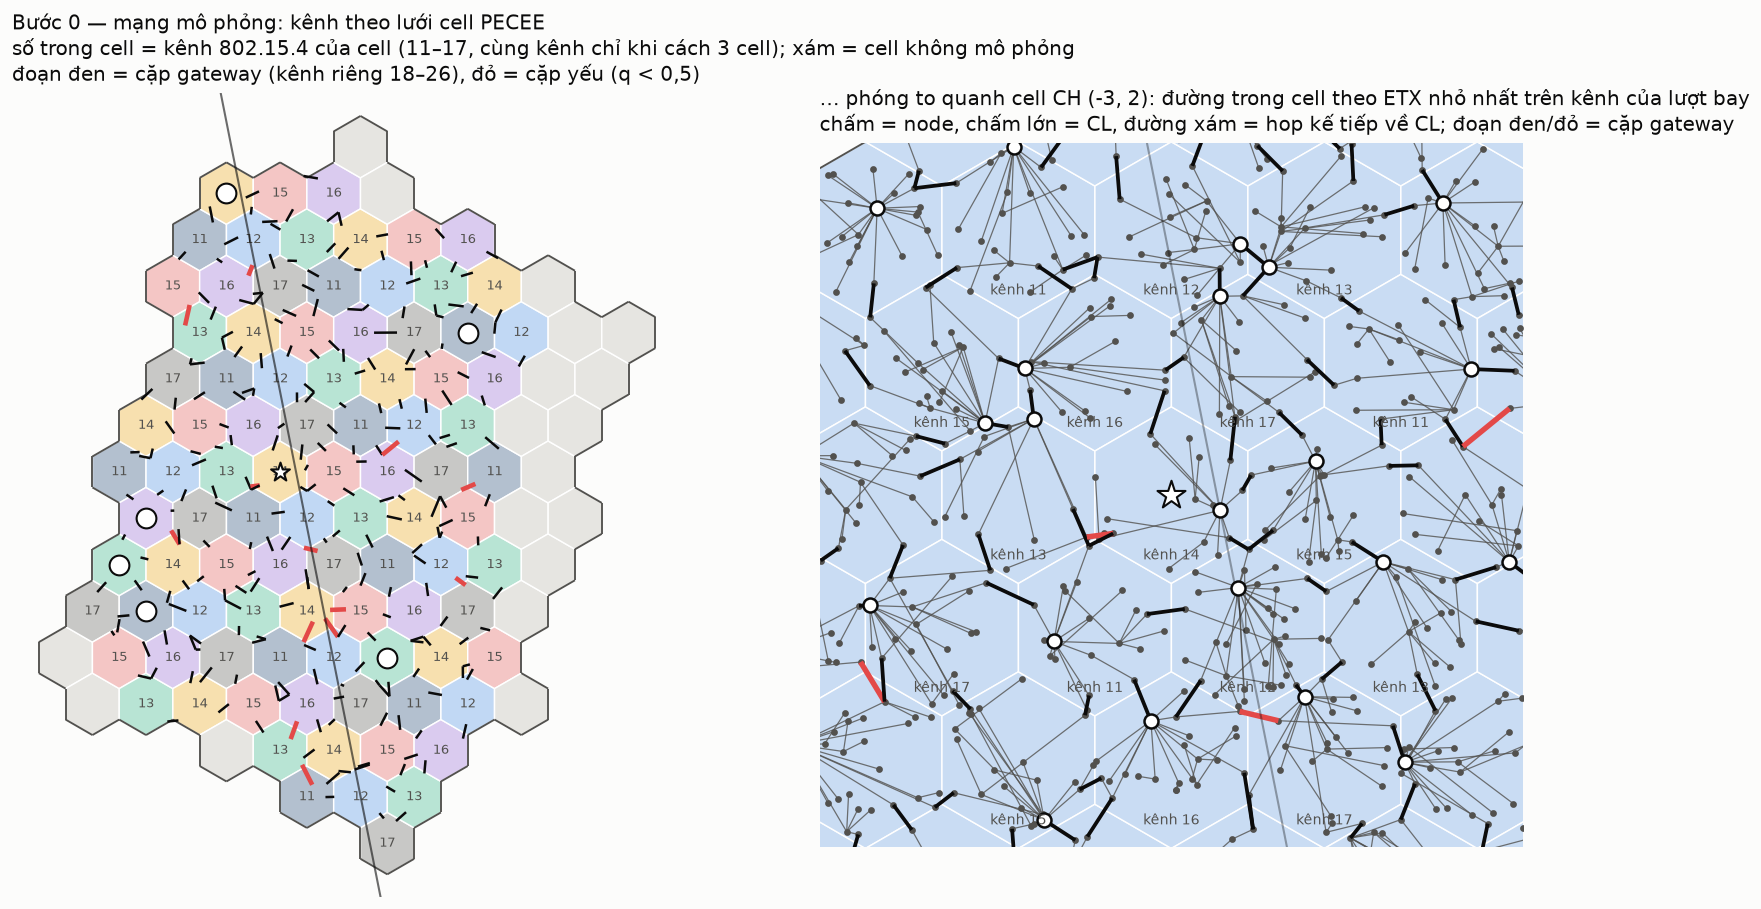
\includegraphics[width=0.82\linewidth,height=0.38\textheight,keepaspectratio]{../../../uav-coop2/docs/figures/ns3-setup.png}
\caption{Pha 0 trong mô phỏng hiện tại. Trái: kênh của mỗi cell
theo lưới 7 màu và các cặp gateway (đoạn đen; đoạn đỏ là cặp yếu). Phải:
phóng to quanh CH, mỗi node nối về CL theo đường có ETX nhỏ nhất.}
\end{figure}

\textbf{Nội dung nghiên cứu.}

\begin{itemize}
\item
  \textbf{Quy tắc chọn R.} R tác động tới mọi lớp phía sau, theo hai
  chiều ngược nhau.

  \begin{itemize}
  \tightlist
  \item
    R lớn: mỗi cell có nhiều node hơn, nên gom nội cell nhiều hop hơn và
    CL tải nặng hơn. Đổi lại, River đi qua ít cell hơn.
  \item
    R nhỏ: phải có đủ node để mỗi cạnh chung luôn có cặp gateway liên
    kết tốt.
  \item
    Ngoài ra, độ rộng River tính theo cell và tỉ lệ $R_{50}$/R cũng thay đổi
    theo R.
  \end{itemize}

  ND0 phát biểu R là nghiệm của một ràng buộc: R nhỏ nhất sao cho mỗi
  cell có ít nhất n\_min node, và mỗi cạnh chung có ít nhất một cặp node
  với xác suất liên kết ≥ q. Sau đó quét R để xem $T^\star$ thay đổi thế nào.
\item
  \textbf{Chi phí dựng và phát kế hoạch.} Pha 0 có hai loại chi phí, xem
  Hình 8.

  \begin{itemize}
  \tightlist
  \item
    Chi phí một lần: trạm gốc gom topo lên (vị trí, năng lực, chất lượng
    liên kết), rồi phát cấu trúc lưới xuống.
  \item
    Chi phí lặp lại trước mỗi nhiệm vụ: phát bảng Seg, vai trò Bank/Ring
    và các đường cell tới từng cell.
  \end{itemize}

  Cả hai sẽ được mô phỏng bằng frame thật và đo theo số node, mật độ và
  kích thước cụm.
\item
  \textbf{Gateway một radio và giới hạn kênh.}

  \begin{itemize}
  \tightlist
  \item
    Thay giả định đa radio bằng bản một radio: node gateway chia thời
    gian giữa kênh cell và kênh cặp, rồi đo River chậm đi bao nhiêu.
  \item
    802.15.4 ở 2,4 GHz chỉ có 16 kênh, nên khi mạng dày sẽ phải dùng lại
    kênh. Cần đo ảnh hưởng của việc này.
  \end{itemize}
\item
  \textbf{Đồng bộ và đánh thức.} Lịch kênh cần đồng hồ chung. Node phải
  thức đúng lúc UAV bay qua, nếu không sẽ phải thức suốt nhiệm vụ. ND0
  thiết kế một cơ chế đánh thức theo lịch bay mà trạm gốc phát trong kế
  hoạch, và tính cả sai số đồng hồ.
\item
  \textbf{Bền vững của cấu trúc.}

  \begin{itemize}
  \tightlist
  \item
    Cạnh không có cặp gateway (qua hồ hoặc vùng thưa) làm hai cell kề
    không nối với nhau.
  \item
    Mỗi cạnh chỉ có một cặp gateway, nên cặp này vừa là điểm hỏng đơn
    vừa là nút cổ chai.
  \item
    CL là điểm nóng năng lượng.
  \end{itemize}

  ND0 xét cặp gateway dự phòng, luân phiên vai trò CL, và cách sửa cấu
  trúc cục bộ khi node hỏng hoặc có node mới.
\item
  \textbf{Liên hệ với tái cấu trúc cụm.} Các thử nghiệm LANE và MEANDER
  trước đây sẽ được đánh giá lại khi chi phí dựng pha 0 đã được tính
  vào.
\end{itemize}

\begin{figure}[htbp]
\centering
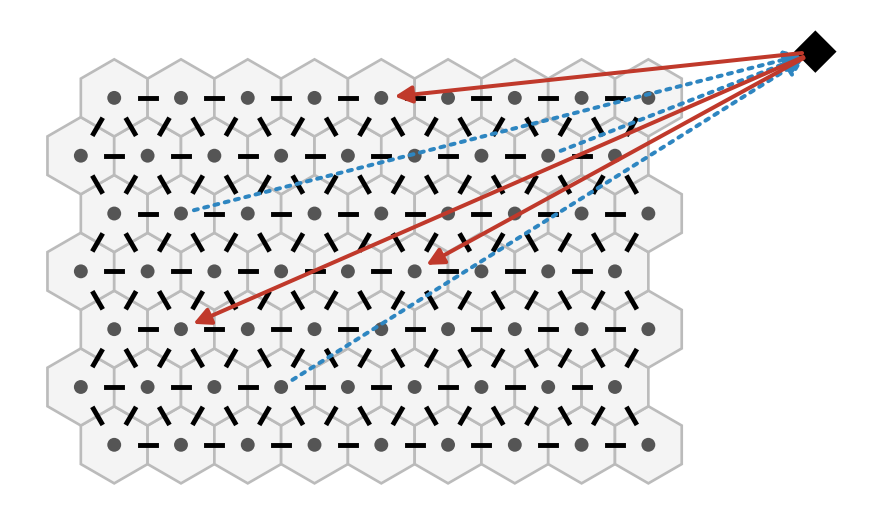
\includegraphics[width=0.82\linewidth,height=0.38\textheight,keepaspectratio]{../../../docs/figures/proposal/nd0-phase0-topology-and-plan-flow.png}
\caption{Hai luồng thông tin của pha 0. Mũi tên chấm: các cell báo
topo lên trạm gốc (hình thoi). Mũi tên liền: trạm gốc phát kế hoạch
xuống trước mỗi nhiệm vụ. Chấm xám là CL; đoạn đen là cặp gateway giữa
hai cell kề.}
\end{figure}

\textbf{Đầu ra.} Quy tắc chọn R; chi phí pha 0 tách thành phần một lần
và phần mỗi nhiệm vụ; độ chậm khi gateway chỉ có một radio; cơ chế đánh
thức. Các kết quả này đi vào phần mô hình của J1 và vào C3.

\subsection{ND1. Mô hình hoá bài toán và các kết quả lý thuyết}

ND1 trả lời RQ1 và là phần lõi của J1.

\textbf{Mô hình chung.} Mọi kết quả dưới đây dựa trên một mô hình hình thức, được chốt trong hai tuần đầu của ND1. Trước khi chốt, mô hình được đối chiếu với \texttt{params.yaml} và với bit nhận thật trong log.

\begin{itemize}\tightlist
\item \textbf{Mạng:} đồ thị cell $G=(V,E)$. Mỗi đỉnh là một cell lục giác bán kính $R$. Mỗi cạnh $e\in E$ là một cặp gateway có dung lượng $c_e$ (gói/s). Tập critical cell là $K\subseteq V$.
\item \textbf{Truy vấn:} $Q$ gói; UAV phát một gói mỗi $\tau$ giây.
\item \textbf{Quỹ đạo:} $\gamma$ là đường bay dự kiến, $\gamma'$ là đường bay thật. Gói $s$ được phát tại $\gamma'(s\tau)$. Độ lệch ngang lớn nhất là $\bar e=\sup_t\lVert\gamma'(t)-\gamma(t)\rVert$.
\item \textbf{Kênh A2G:} một node nhận được gói với xác suất $p(d)$, trong đó $d$ là khoảng cách ngang tới điểm UAV phát gói đó. $p(d)$ lấy từ mô hình hai đoạn kèm fading Nakagami, đặc trưng bởi $R_{50}$.
\item \textbf{Giả định A1:} các lần nhận gói độc lập với nhau. Giả định này lạc quan và được nêu rõ trong bài.
\item \textbf{Thời gian nhiệm vụ:} $T^\star=T_{\text{bay}}+T_{\text{đất}}+T_{\text{đối sánh}}+T_{\text{LoRa}}+T_{\text{pha 2}}$. Các kết quả chỉ so sánh hai thành phần đầu; các thành phần còn lại chung cho mọi phương án.
\end{itemize}

\textbf{Các kết quả dự kiến.} Các phát biểu dưới đây là dạng dự kiến, sẽ được chỉnh khi chứng minh.

\begin{lemma}[Độ khó]\label{lem:np}
Bài toán chọn quỹ đạo và kế hoạch để $T^\star$ nhỏ nhất là NP-khó.
\end{lemma}
\noindent\emph{Hướng chứng minh.} Quy từ DTSP-N: cho $Q$ rất nhỏ và dung lượng mặt đất vô hạn, bài toán chỉ còn tìm tour Dubins ngắn nhất qua đĩa các CH.

\begin{theorem}[Điểm giao giữa hợp tác và bay vòng]\label{thm:A}
Gọi $p_k$ là xác suất critical cell $k$ nhận được một gói ở vị trí thuận lợi nhất của UAV, $n_k$ là số gói $k$ đã nhận khi UAV bay ngang, và $\varepsilon$ là phần dư của fountain code. Khi đó
\[
T_{\mathrm{FC}}\;\ge\;T^{\mathrm{FC}}_{\text{tour}}+\sum_{k\in K}\tau\Big[\frac{Q(1+\varepsilon)}{p_k}-n_k\Big]^+,
\qquad
T_{\mathrm{River}}\;\le\;T^{\text{1 lượt}}_{\text{tour}}+T_{\text{đất}},
\]
với $T_{\text{đất}}$ bị chặn như ở Mệnh đề~\ref{prop:D}. River nhanh hơn FC khi vế phải thứ nhất lớn hơn vế phải thứ hai. Hơn nữa, $T_{\mathrm{FC}}/T_{\mathrm{River}}$ tăng theo cỡ $1/p_{\min}$ khi $R_{50}$ giảm, và tiến về $1$ khi $R_{50}$ lớn hơn bề rộng cụm.
\end{theorem}
\noindent Định lý giải thích hiện tượng đã đo: ở kênh open hai phương án gần ngang nhau, ở r200/r100 River nhanh hơn 49–72\,\%. Nó cũng cho người thiết kế một quy tắc: khi nào nên đầu tư vào hợp tác mặt đất.

\setcounter{proposition}{1}
\begin{proposition}[Ngưỡng lệch của takeover]\label{prop:B}
Gọi $w$ là khoảng cách lớn nhất từ điểm phát tới tập $a\cup N(a)$ (SPINE cell $a$ và các cell kề), sao cho tập này vẫn có node nhận gói với xác suất không nhỏ hơn $p_{\min}$; $w$ phụ thuộc $R$ và $R_{50}$.
\begin{enumerate}
\item[(i)] Nếu $\bar e< w-\tfrac{\sqrt3}{2}R$ thì takeover không phải kích hoạt, với xác suất ít nhất $1-\delta$.
\item[(ii)] Nếu $\bar e\ge w$ thì mọi gói thiếu của $\mathrm{Seg}(a)$ nằm trong $h(\bar e)=\big\lceil(\bar e-w)/(\sqrt3R)\big\rceil+1$ hop cell tính từ $a$. Vòng hỏi trong bán kính $h(\bar e)$ là đủ, và số frame của nó có chặn trên tương ứng.
\end{enumerate}
\end{proposition}
\noindent Mệnh đề giải thích vì sao không có lần kích hoạt nào ở $\sigma=50$\,m nhưng có ở $\sigma=100$\,m. Bán kính hỏi 3 hop trở thành một hệ quả thay vì một con số chọn tay (Hình~9).

\begin{figure}[htbp]
\centering
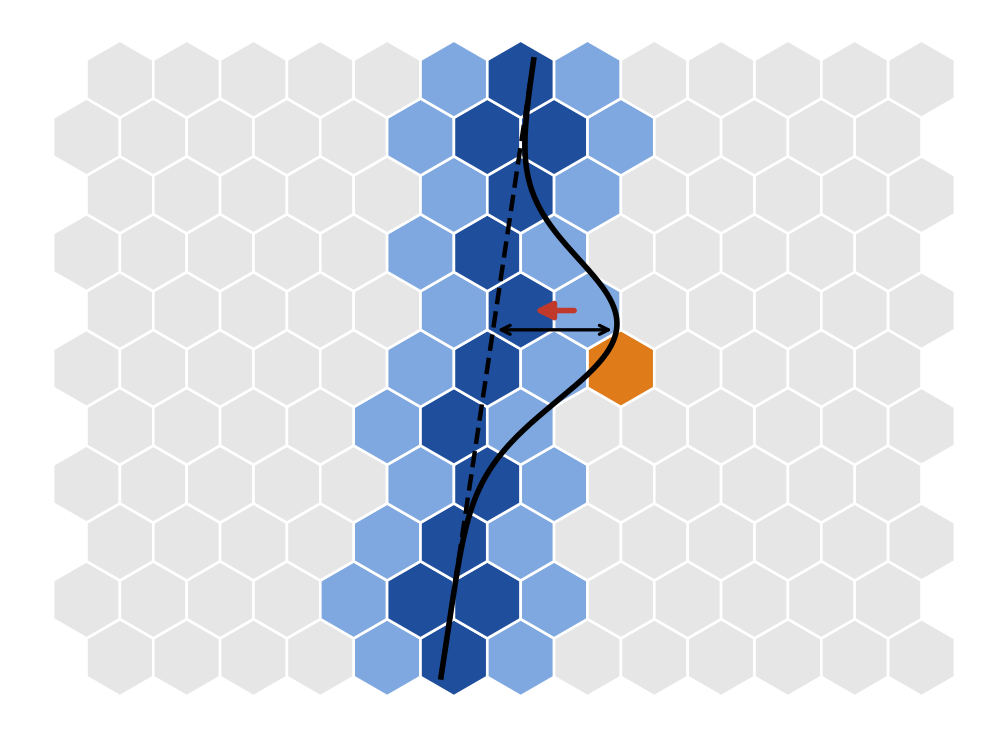
\includegraphics[width=0.82\linewidth,height=0.38\textheight,keepaspectratio]{../../../docs/figures/proposal/prop-b-deviation-threshold.png}
\caption{Mệnh đề B. Đường đứt: quỹ đạo dự kiến qua các SPINE cell
(xanh đậm). Xanh nhạt: vùng mà bước sửa từ cell kề còn phủ được. Đường
liền: quỹ đạo thật lệch một đoạn e (mũi tên hai đầu). Khi e vượt ngưỡng,
gói rơi vào cell ngoài vùng đó (cam) và takeover phải kéo về (mũi tên
đỏ).}
\end{figure}


\setcounter{proposition}{3}
\begin{proposition}[Cận dưới thời điểm sẵn sàng]\label{prop:D}
Với mọi giao thức phân phối dưới mặt đất,
\[
T_{\text{đất}}\;\ge\;\max_{k\in K}\;\max_{S}\;\frac{\mathrm{thiếu}_k(S)}{c(S)}\;+\;h_{\min}(k)\,t_{\text{hop}},
\]
trong đó $S$ chạy trên các lát cắt tách $k$ khỏi nơi giữ dữ liệu, $c(S)$ là tổng dung lượng các cạnh của lát cắt, và $h_{\min}(k)$ là số hop tối thiểu tới $k$.
\end{proposition}
\noindent Sẽ thử chứng minh River đạt cận này nhân một hằng số khi các cặp gateway dùng kênh riêng. Nếu chưa chứng minh được, chỉ báo khoảng cách đo được.

\setcounter{theorem}{2}
\begin{theorem}[Giá trị thông tin của kế hoạch, có điều kiện]\label{thm:C}
Gọi $X$ là mẫu nhận gói (node nào giữ gói nào). Với lớp giao thức chỉ dùng thông tin cục bộ, chi phí điều khiển của mọi giao thức khám phá là $\Omega(H(X))$ bit. Chi phí của River kèm takeover là $O\big(H(X\mid\text{kế hoạch})\big)$, và đại lượng này tăng theo $\bar e$.
\end{theorem}
\noindent Định lý~\ref{thm:C} chỉ đưa vào J1 nếu thử nghiệm ở tuần 9–10 cho thấy $H(X\mid\text{kế hoạch})\ll H(X)$ ở quỹ đạo danh nghĩa, và đại lượng này tăng cùng chiều với số frame điều khiển đo được. Nếu không, nó để thành hướng mở.

\textbf{Kiểm chứng.} Mỗi kết quả có một script trong
\texttt{uav-l2/tools/theory/} và một hình đặt đường lý thuyết chồng lên
số liệu ns-3 sẵn có. Giai đoạn này gần như không cần chạy ns-3 mới.

\begin{itemize}
\tightlist
\item
  A: tỉ số T\_FC/T\_River theo $R_{50}$, so với các ô của C4.
\item
  B: số lần kích hoạt takeover và số hop tới cell giữ gói theo e, so với
  WND và TKO.
\item
  D: thời điểm sẵn sàng đo được so với cận, theo từng cụm. c\_e lấy từ
  thông lượng thực đo của các cặp gateway.
\item
  C: entropy ước lượng từ bit nhận, đặt cạnh số frame điều khiển của DLG
  và TKO.
\end{itemize}

\subsection{ND2. Giao thức River và takeover}

\textbf{Mục tiêu.} ND2 đưa River từ bản chạy được trong mô phỏng thành
giao thức dùng được ngoài thực tế. Nó gỡ các giả định lạc quan đã nêu ở
mục 4.6, và trả lời RQ2 và một phần RQ3.

\textbf{Takeover theo tọa độ trong header.} Mỗi gói UAV phát mang tọa độ
thật của UAV. Sau khi gom nội cell, cell nào nhận được gói phát ngay
trên mình nhưng gói đó thuộc đoạn của một SPINE cell khác sẽ gửi một báo
cáo ngắn: chỉ một đoạn chỉ số {[}min, max{]} tới SPINE cell đó. SPINE
cell kéo phần còn thiếu thẳng từ cell này; bước hỏi lan chỉ để dự phòng
(Hình 10).

Khi bay đúng kế hoạch, cơ chế này không phát frame nào. Nó sẽ được mô
phỏng đầy đủ và so với hai bản đã có: SPINE cell tự hỏi lan, và oracle.
Chỉ số so sánh là thời điểm sẵn sàng, số frame điều khiển, và tỉ lệ
critical cell nhận đủ theo độ lệch e.

\begin{figure}[htbp]
\centering
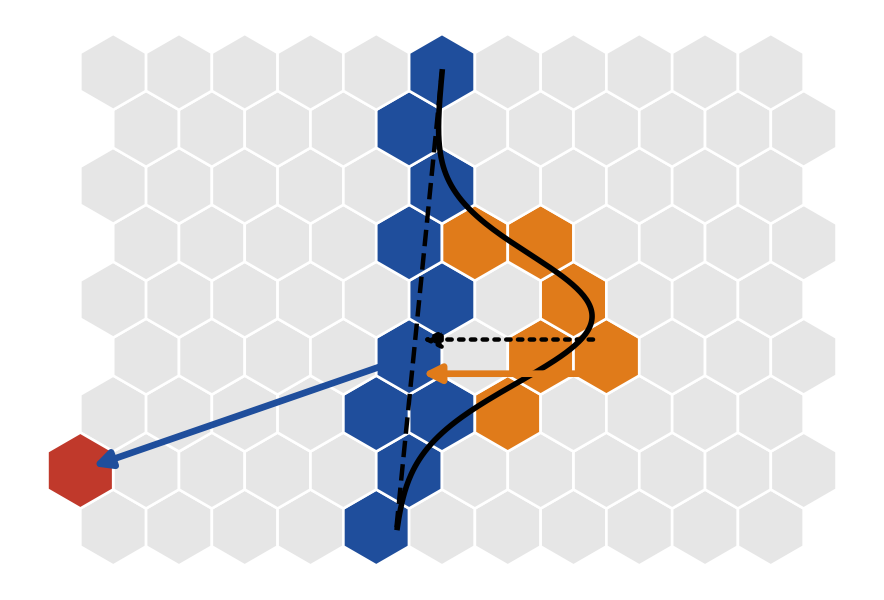
\includegraphics[width=0.82\linewidth,height=0.38\textheight,keepaspectratio]{../../../docs/figures/proposal/nd2-takeover-header-report.png}
\caption{Takeover theo tọa độ trong header. Đường đứt là quỹ đạo
dự kiến, đi qua các SPINE cell (xanh đậm); đường liền là quỹ đạo thật.
Các cell cam nằm dưới quỹ đạo thật và nhận gói thuộc đoạn của SPINE
cell. Mũi tên chấm: báo cáo từ cell cam tới SPINE cell. Mũi tên cam: dữ
liệu kéo về. Mũi tên xanh: SPINE cell tiếp tục phục vụ critical cell
(đỏ) theo kế hoạch.}
\end{figure}

\textbf{Gỡ các giả định lạc quan.}

\begin{itemize}
\tightlist
\item
  \textbf{Kênh lệch mô hình.} Trạm gốc lập kế hoạch bằng một mô hình
  kênh, nhưng mô phỏng chạy trên một kênh khác: lệch số mũ suy hao, lệch
  $R_{50}$, có tương quan theo thời gian. Từ đó đo River suy giảm thế nào, và
  takeover bù được bao nhiêu.
\item
  \textbf{Phân phối chồng với lượt bay.} Cho phép cụm vừa được bay qua
  bắt đầu phân phối trong lúc UAV phát cho cụm kế bên. Mô phỏng cả nhiễu
  giữa lưu lượng mặt đất và gói UAV.
\item
  \textbf{Lịch ngủ thật.} Node tắt radio theo kế hoạch thay vì tính năng
  lượng sau khi chạy. Đo năng lượng thật và kiểm tra River vẫn đúng hạn.
\item
  \textbf{Gateway một radio.} Dùng kết quả của ND0 để chạy River với
  gateway chia thời gian giữa hai kênh.
\end{itemize}

\textbf{River dùng fountain code.} Mỗi ảnh được mã thành một khối riêng.
SPINE cell, Bank và Ring phụ trách các dải ID gói mã riêng. Cell đã giải
mã được ảnh thì tự sinh gói mã mới, nên không gây trùng lặp và bên nhận
chỉ cần báo còn thiếu bao nhiêu. So sánh với River vận chuyển gói gốc,
về thời gian, số frame và nhu cầu dùng takeover.

\textbf{Các câu hỏi phụ đã ghi nhận.}

\begin{itemize}
\tightlist
\item
  Độ rộng River tối ưu theo $R_{50}$ và mật độ.
\item
  Cách ghép các Ring khi hai critical cell nằm cạnh nhau.
\item
  Cách dựng Bank theo pháp tuyến cục bộ khi SPINE cong.
\end{itemize}

\textbf{So sánh đầy đủ với Deluge-lite.} Bản Deluge mạnh hơn: page không
theo thứ tự, NACK theo bitmap, cùng lượt bay LM-Tour. Hai cấu hình
Trickle được tinh chỉnh trước, rồi cố định trước khi chạy chính.

\textbf{Đầu ra.} Giao thức River hoàn chỉnh, gồm takeover theo header và
biến thể fountain code, kèm số đo dưới các giả định thực tế hơn. Đây là
phần giao thức của J1, và là nội dung của C1, C2, C5.

\subsection{ND3. Thiết kế quỹ đạo và surrogate}

\textbf{Mục tiêu.} ND3 làm cho LM-Tour có cơ sở vững hơn và tổng quát
hơn. Nó trả lời RQ4.

\textbf{Bộ dự đoán thời gian River.}

\begin{itemize}
\tightlist
\item
  \textbf{Kiểm định theo bản đồ.} Học trên một tập bản đồ, kiểm trên bản
  đồ chưa thấy. Báo sai số theo từng mức kênh.
\item
  \textbf{Đặc trưng.} Thêm đặc trưng về hình dạng cụm (độ dài SPINE, bề
  rộng, số critical cell ngoài River) và về chất lượng cặp gateway.
\item
  \textbf{Mô hình giải tích.} So bộ dự đoán với mô hình giải tích từ
  ND1, để biết phần nào giải thích được bằng lý thuyết và phần nào chỉ
  học được từ dữ liệu.
\end{itemize}

\begin{figure}[htbp]
\centering
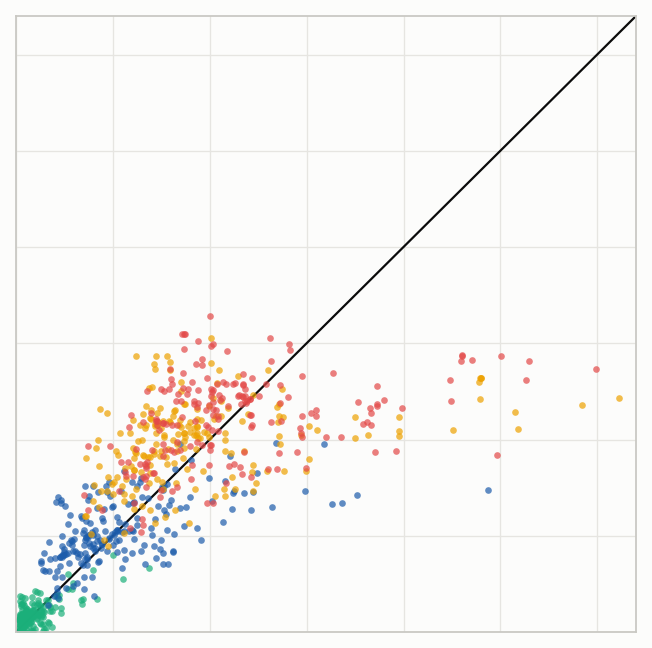
\includegraphics[width=0.82\linewidth,height=0.38\textheight,keepaspectratio]{../../../uav-l2/docs/figures/lm-surrogate-pred-vs-ns3.png}
\caption{Bộ dự đoán thời gian River: mỗi chấm là một critical cell
(812 cell, 3 bản đồ × 4 kênh). Trục ngang là thời gian ns-3 đo được,
trục dọc là thời gian dự đoán.}
\end{figure}

\textbf{LM-Tour.}

\begin{itemize}
\tightlist
\item
  \textbf{Bán kính đĩa ξ.} Chọn ξ theo $R_{50}$ bằng quy tắc thay cho dò tay.
\item
  \textbf{Điều kiện dừng.} Làm rõ khi nào việc uốn về landmark đã bão
  hoà. Nếu thay lợi ích bằng một hàm phủ có trọng số, bước uốn tham lam
  có thể có bảo đảm xấp xỉ. Đây là định lý tuỳ chọn, chỉ làm nếu ND1 còn
  thời gian.
\item
  \textbf{Động học và năng lượng.} Đưa ràng buộc gia tốc 1 g và năng
  lượng UAV (mô hình có số hạng gia tốc, đã đối chiếu hệ số c₁, c₂) vào
  hàm mục tiêu.
\item
  \textbf{CH ở vị trí bất kỳ.} Đánh giá khi CH không phải node tốt nhất,
  vì thử trước đây cho thấy kết quả kém đi rõ.
\end{itemize}

\textbf{Nhiều UAV ở pha 1.} Chia các cụm cho nhiều UAV để $T^\star$ nhỏ nhất,
có xét chồng lấn thời gian phân phối mặt đất giữa các cụm.

\textbf{Đầu ra.} LM-Tour có quy tắc chọn tham số, bộ dự đoán đã kiểm
định trên bản đồ mới, và bản nhiều UAV. Đây là phần quỹ đạo của J1, và
là nội dung của C4.

\subsection{ND4. Đánh giá mô phỏng quy mô lớn}

\textbf{Mục tiêu.} ND4 cho J1 một bộ số liệu đủ rộng và đủ chặt để kết
luận không phụ thuộc vào một bản đồ hay một seed. Nó trả lời phần còn
lại của RQ3.

\textbf{Thiết kế chiến dịch.}

\begin{itemize}
\tightlist
\item
  Ba cỡ bản đồ (8, 12, 15 cụm), mỗi cỡ 10 bản đồ, mỗi bản đồ đủ 10 seed.
\item
  Bốn mức kênh.
\item
  Các phương án: LM-Tour + River (đề xuất), CHORD + River, DTSP-N +
  River, FC + DTSP-N, Deluge-lite.
\item
  Binary được chốt trước khi chạy và không đổi trong suốt chiến dịch.
\end{itemize}

\textbf{Độ bền vững.} Bốn loại sai lệch được thêm vào lần lượt, mỗi loại
một trục:

\begin{itemize}
\tightlist
\item
  gió lệch quỹ đạo, σ 50--200 m, đủ seed, chỉ giữ các quỹ đạo bay được
  (gia tốc ≤ 1 g);
\item
  5--20 \% node hỏng ngẫu nhiên sau khi đã lập kế hoạch;
\item
  kênh thật khác mô hình lập kế hoạch;
\item
  vật cản, nếu đưa vào phạm vi.
\end{itemize}

Với mỗi trục, báo $T^\star$, tỉ lệ critical cell nhận đủ và chi phí sửa lỗi
(frame takeover).

\textbf{Khả năng mở rộng.} Đo thời gian mô phỏng theo số node, tới cụm
khoảng 2 000 node. Nếu ns-3 chạy quá chậm, cân nhắc mô phỏng song song
(MPI), hoặc giản lược MAC ở phần không nằm trên đường găng.

\textbf{Thống kê.} Mọi so sánh đều ghép cặp. Báo CI 95 \% theo seed và
số seed mà đề xuất thắng. Mỗi kết quả lý thuyết của ND1 có hình đặt
đường lý thuyết chồng lên số liệu của chiến dịch này.

\textbf{Đầu ra.} Bảng kết quả chính và bảng độ bền vững của J1, cùng bộ
dữ liệu công khai.

\subsection{ND5. Kiểm chứng trên phần cứng (nếu có điều kiện)}

\textbf{Mục tiêu.} ND5 kiểm tra kết quả mô phỏng còn giữ được bao nhiêu
trên phần cứng thật, và dùng số đo thật để hiệu chỉnh mô hình kênh. Nó
trả lời RQ6. Kiểm chứng đi theo ba bậc, chi phí tăng dần.

\begin{itemize}
\tightlist
\item
  \textbf{Bậc 1: testbed 802.15.4.}

  \begin{itemize}
  \tightlist
  \item
    Phần cứng: FIT IoT-LAB, hoặc 20--50 node nRF52840 / CC2652 trong
    phòng thí nghiệm, cộng vài máy cỡ Raspberry Pi làm critical cell.
  \item
    Firmware: Contiki-NG, RIOT hoặc Zephyr.
  \item
    Thí nghiệm: chạy River với lịch kênh thật; một node phát di động
    đóng vai UAV.
  \item
    Đo PER G2G, thời điểm sẵn sàng và năng lượng, rồi so với ns-3 trên
    cùng topo.
  \end{itemize}
\item
  \textbf{Bậc 2: PX4 SITL ghép ns-3.} Kiểm quỹ đạo CHORD và LM-Tour với
  động học bay thật của UAV cánh bằng: giới hạn góc nghiêng, ảnh hưởng
  của gió, sai số GPS ghi vào header.
\item
  \textbf{Bậc 3: bay thật trên một cụm khoảng 30 node.}

  \begin{itemize}
  \tightlist
  \item
    Phần cứng: UAV có Pixhawk và radio 802.15.4 gắn ngoài.
  \item
    Điều kiện: chỉ làm khi có giấy phép bay và bãi thử.
  \end{itemize}
\end{itemize}

Bậc 1 và 2 đã đủ cho một bài tạp chí. Bậc 3 là phần thêm nếu có điều
kiện.

\textbf{Đầu ra.} Số đo PER và năng lượng thật, mô hình kênh G2G đã hiệu
chỉnh, và so sánh giữa phần cứng và mô phỏng. Đây là nội dung chính của
J2.

\subsection{ND6. Pha 2: lịch xác minh}

\textbf{Mục tiêu.} ND6 đưa pha 2 từ một mô hình thời gian đơn giản thành
một bài toán lập lịch có cơ sở, để $T^\star$ phản ánh đúng nhiệm vụ đầu--cuối.
Nó trả lời RQ5.

\textbf{Mô hình.} Sau khi đối sánh, mỗi critical cell gửi điểm cao nhất
về trạm gốc qua LoRa. Kênh này có giới hạn chu kỳ phát, nên các báo cáo
về muộn khác nhau. Đội UAV cánh quay bay tới các cell nghi vấn. Ở mỗi
cell, UAV hover để tải tệp xác minh lớn và chờ đối sánh. Nhiệm vụ xong
khi đã xác minh cell có điểm cao nhất.

\textbf{Nội dung nghiên cứu.}

\begin{itemize}
\tightlist
\item
  \textbf{Thứ tự thăm.} So thăm theo điểm, theo TSP thuần, và theo một
  tiêu chí kết hợp điểm với quãng bay (Hình 12). Có xét việc điểm số đến
  muộn qua LoRa: đội 2 có nên xuất phát trước khi nhận đủ báo cáo không.
\item
  \textbf{Liên kết với lớp 1.} Dùng mô hình điểm khớp và trọng số manh
  mối để tính xác suất mục tiêu thật nằm ở mỗi cell. Từ đó tính xác suất
  tìm thấy mục tiêu theo thời gian, thay vì chỉ một con số $T^\star$.
\item
  \textbf{Nhiều mục tiêu, nhiều UAV.} Mở rộng cho nhiều mục tiêu hoặc
  mục tiêu di chuyển để lại vệt qua nhiều camera, và cho nhiều UAV xác
  minh.
\end{itemize}

\begin{figure}[htbp]
\centering
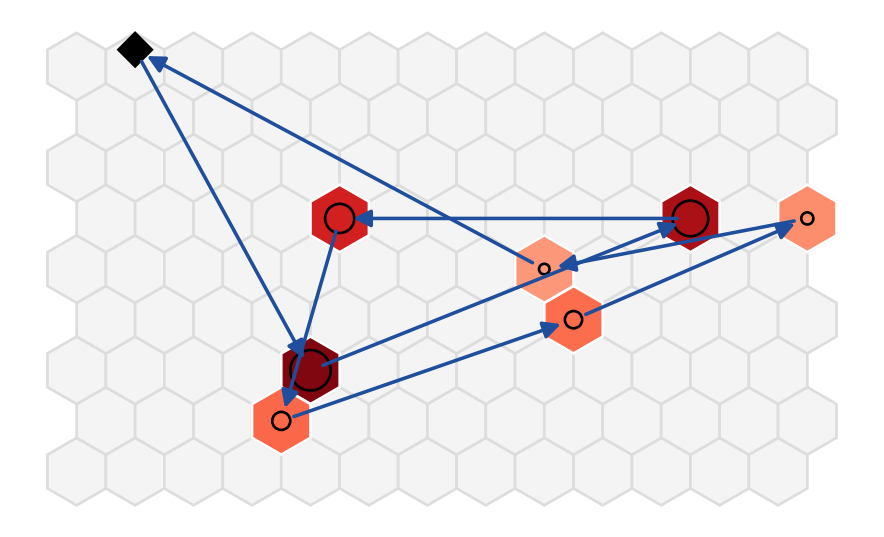
\includegraphics[width=0.82\linewidth,height=0.38\textheight,keepaspectratio]{../../../docs/figures/proposal/nd6-phase2-score-ordered-visits.png}
\caption{Pha 2: các cell nghi vấn tô đậm và vòng tròn lớn theo
điểm số. UAV cánh quay xuất phát từ trạm gốc (hình thoi) và thăm các
cell theo thứ tự điểm giảm dần.}
\end{figure}

\textbf{Đầu ra.} Thuật toán lập lịch xác minh và mô hình xác suất tìm
thấy theo thời gian. Phần này đi vào mô hình đầu--cuối của J1, ở mức mô
hình, chưa chạy ns-3.

\section{Kết quả dự kiến và sản phẩm}

\subsection{Bài báo}

Ưu tiên của giai đoạn sau ICC là \textbf{bài tạp chí}: một bài chính
trình bày lời giải đầy đủ, và nếu kịp, một bài thứ hai về triển khai.
Các kết quả nhỏ, tự đứng được, sẽ được tách thành bài hội nghị rank B
hoặc A- (cỡ ICC trở xuống).

Tách bài phải tuân theo chính sách của IEEE: bài tạp chí mở rộng từ bài
hội nghị cần có phần mới đáng kể, nên mỗi bài hội nghị chỉ dùng một kết
quả hẹp và không lặp lại phần lõi của bài tạp chí.

\textbf{Bài tạp chí}

\textbf{J1. Bài chính: lời giải đầy đủ cho phát truy vấn bằng UAV cánh
bằng} (nơi gửi: IEEE TMC hoặc IEEE IoT-J, phương án dự phòng IEEE TVT
\textbf{{[}cần chốt{]}}; nộp khoảng 06--07/2027). Bài là bản mở rộng có
hệ thống từ bài ICC, gồm năm phần.

\begin{itemize}
\tightlist
\item
  \textbf{Mô hình và lý thuyết (ND1).} Bài toán đầu--cuối cho ba pha,
  kèm:

  \begin{itemize}
  \tightlist
  \item
    bổ đề NP-khó;
  \item
    định lý điểm giao giữa hợp tác mặt đất và bay vòng (định lý A): khi
    nào River thắng FC, theo $R_{50}$, số critical cell và kích thước truy
    vấn;
  \item
    mệnh đề ngưỡng lệch của takeover (định lý B);
  \item
    cận dưới của thời điểm sẵn sàng theo lát cắt nhỏ nhất của đồ thị
    cell (định lý D).
  \item
    Mỗi kết quả lý thuyết đều có hình đặt đường lý thuyết chồng lên số
    liệu ns-3.
  \end{itemize}
\item
  \textbf{Giao thức (ND2).} River hoàn chỉnh, gồm:

  \begin{itemize}
  \tightlist
  \item
    takeover theo tọa độ trong header;
  \item
    năng lượng có lịch ngủ thật được mô phỏng;
  \item
    bản một radio cho gateway, bên cạnh bản đa radio;
  \item
    so sánh đầy đủ với Deluge-lite.
  \end{itemize}
\item
  \textbf{Quỹ đạo (ND3).} CHORD và LM-Tour, với bộ dự đoán đã kiểm định
  trên bản đồ chưa thấy.
\item
  \textbf{Pha 0 và pha 2 ở mức mô hình.} Chi phí dựng lưới và phát kế
  hoạch; lịch đội xác minh có hover, tải tệp lớn và trễ LoRa.
\item
  \textbf{Đánh giá quy mô lớn (ND4).} Ba cỡ bản đồ, mỗi cỡ 10 bản đồ, đủ
  seed. Độ bền vững trước gió, node hỏng và sai lệch mô hình kênh.
\end{itemize}

Đóng góp mà bài này nhắm tới là: một kiến trúc có bảo đảm hình thức, quy
tắc thiết kế cho biết khi nào hợp tác mặt đất đáng giá, và đánh giá
packet-level ở quy mô lớn.

\textbf{J2. Bài triển khai: từ mô phỏng tới phần cứng} (nơi gửi: IEEE
IoT-J hoặc ACM TOSN \textbf{{[}cần chốt{]}}; khoảng cuối 2027, nếu ND5
kịp). Nội dung gồm:

\begin{itemize}
\tightlist
\item
  dựng pha 0 bằng frame thật;
\item
  River và takeover trên testbed 802.15.4;
\item
  PX4 SITL ghép ns-3 để kiểm quỹ đạo;
\item
  so sánh PER, thời điểm sẵn sàng và năng lượng giữa phần cứng và mô
  phỏng;
\item
  hiệu chỉnh mô hình kênh G2G từ số đo thật.
\end{itemize}

\textbf{Bài hội nghị tách từ kết quả nhỏ}

Danh sách hội nghị dưới đây là gợi ý theo chủ đề. Rank cần kiểm tra lại
theo CORE hoặc danh mục của đơn vị trước khi chọn.

\begin{itemize}
\tightlist
\item
  \textbf{C1. River tự thích ứng với sai lệch quỹ đạo.} Takeover tuần tự
  và takeover theo tọa độ trong header, so với oracle và với River không
  sửa lỗi. Thí nghiệm gió σ 50--200 m, kèm ngưỡng lệch ở định lý B. Nơi
  gửi: IEEE WCNC hoặc IEEE VTC. Đây là bài sẵn nhất, vì số liệu gần đủ.
\item
  \textbf{C2. Lập kế hoạch hay khám phá trong phổ tán dữ liệu.} River so
  với Deluge-lite, về số frame, năng lượng và node nóng nhất. Có thể kèm
  khung "giá trị thông tin của kế hoạch" (định lý C, ở dạng sơ bộ). Nơi
  gửi: DCOSS-IoT, IEEE MASS hoặc IEEE ISCC.
\item
  \textbf{C3. Tổ chức mạng theo lưới cell cho phân phối có kế hoạch.}
  Quy tắc chọn R theo mật độ, chi phí dựng và bảo trì pha 0, gateway một
  radio so với đa radio, giới hạn 16 kênh. Nơi gửi: IEEE PIMRC hoặc IEEE
  LCN.
\item
  \textbf{C4. Lập quỹ đạo UAV nhờ bộ dự đoán học từ mô phỏng.} LM-Tour,
  bộ dự đoán dạng cây và khả năng tổng quát hoá sang bản đồ mới. Nơi
  gửi: IEEE VTC, hoặc workshop về học máy cho mạng tại ICC/GLOBECOM.
\item
  \textbf{C5. River dùng fountain code.} Phân công theo dải ID, cell đã
  giải mã sinh gói mới, so sánh với River gói gốc. Nơi gửi: IEEE WCNC
  hoặc workshop tại ICC.
\end{itemize}

Thứ tự đề xuất:

\begin{enumerate}
\def\labelenumi{\arabic{enumi}.}
\tightlist
\item
  Nộp C1 sớm nhất, khoảng đầu 2027.
\item
  Sau đó C2 và C4.
\item
  C3 và C5 khi các nội dung tương ứng xong.
\end{enumerate}

J1 sẽ dẫn các bài hội nghị này và nêu rõ phần mới của nó.

\subsection{Mã nguồn và dữ liệu}

Bộ mô phỏng ns-3 (\texttt{uav-coop/}, \texttt{uav-coop2/}) và công cụ
lập quỹ đạo (\texttt{uav-l2/tools/}) sẽ được công khai khi J1 được chấp
nhận. Kèm theo là bộ dữ liệu bản đồ, lượt bay, bit nhận và kết quả các
chiến dịch dưới dạng CSV, cùng tệp tham số \texttt{params.yaml}, để
người khác tái lập được mọi bảng và hình.

\section{Kế hoạch thực hiện}

\subsection{Các giai đoạn}

Kế hoạch xoay quanh một mục tiêu: \textbf{nộp J1 vào khoảng tháng
07/2027.} Mỗi giai đoạn hoàn thành một phần của J1, theo đúng thứ tự các
mục của bài. Bài hội nghị chỉ là sản phẩm phụ: khi một phần của J1 đã có
kết quả hẹp, tự đứng được, thì tách ra nộp, không mở thêm việc riêng cho
chúng. J2 và các nội dung phần cứng để sau khi J1 đã nộp. Kế hoạch tính
từ tháng 12/2026.

\textbf{Giai đoạn 1 (12/2026--02/2027): phần mô hình và lý thuyết của J1
(ND1).}

\begin{itemize}
\tightlist
\item
  Phát biểu bài toán đầu--cuối và chứng minh bổ đề NP-khó.
\item
  Phát biểu và chứng minh định lý A (điểm giao giữa hợp tác và bay
  vòng), mệnh đề B (ngưỡng lệch của takeover) và cận dưới D, trên mô
  hình đơn giản.
\item
  Vẽ đường lý thuyết chồng lên số liệu ns-3 sẵn có (C4, WND, TKO) để
  kiểm tra sớm.
\item
  Song song: trả lời phản biện ICC.
\end{itemize}

\textbf{Chi tiết giai đoạn 1 (ND1, 12 tuần).}

\begin{longtable}[]{@{}lll@{}}
\toprule\noalign{}
Tuần & Việc & Mốc \\
\midrule\noalign{}
\endhead
\bottomrule\noalign{}
\endlastfoot
1--2 & Mô hình, ký hiệu, giả định; bổ đề L1 & Chốt mô hình \\
3--5 & Định lý A và kiểm chứng & A xong \\
5--7 & Mệnh đề B và kiểm chứng & B xong \\
7--9 & Mệnh đề D và kiểm chứng & D xong \\
9--10 & Thử nghiệm quyết định cho C & Làm hoặc bỏ C \\
10--12 & Viết mục System model (khoảng 2 trang) và Analysis (3--4 trang)
của J1, rà soát, thử phản ví dụ & Bản nháp hoàn chỉnh \\
\end{longtable}

Nếu chỉ có 2 tháng: bỏ C (để sau J1) và viết dần theo từng mốc. Thứ tự
ưu tiên khi thiếu thời gian là A, B, L1, D.

\textbf{Giai đoạn 2 (01--04/2027): phần giao thức của J1 (ND2).} Giải
quyết các hạn chế về tính thực tế đã nêu ở mục 4.6:

\begin{itemize}
\tightlist
\item
  takeover theo tọa độ trong header;
\item
  gateway một radio;
\item
  lịch ngủ được mô phỏng thật;
\item
  kênh thật lệch khỏi mô hình lập kế hoạch;
\item
  cho phép phân phối mặt đất bắt đầu trong lúc UAV còn bay qua cụm kế
  bên.
\item
  Hoàn tất so sánh với Deluge-lite.
\item
  \textbf{Sản phẩm phụ:} khoảng 03/2027, nếu phần takeover đã đủ thì nộp
  C1.
\end{itemize}

\textbf{Giai đoạn 3 (03--05/2027): phần quỹ đạo, pha 0 và pha 2 của J1
(ND3 và các mô hình liên quan).}

\begin{itemize}
\tightlist
\item
  Kiểm định bộ dự đoán trên bản đồ chưa thấy, và hoàn thiện LM-Tour.
\item
  Mô hình chi phí pha 0: quy tắc chọn R, gom topo và phát kế hoạch.
\item
  Mô hình lịch đội xác minh ở pha 2.
\item
  \textbf{Sản phẩm phụ:} C4 nếu phần bộ dự đoán đủ mới.
\end{itemize}

\textbf{Giai đoạn 4 (04--06/2027): phần đánh giá của J1 (ND4).}

\begin{itemize}
\tightlist
\item
  Đóng băng binary.
\item
  Chạy chiến dịch cuối: ba cỡ bản đồ, mỗi cỡ 10 bản đồ, đủ seed, cùng
  các kịch bản bền vững.
\item
  Viết bản thảo hoàn chỉnh và rà soát nội bộ.
\end{itemize}

\textbf{Giai đoạn 5 (07/2027): nộp J1.}

\begin{itemize}
\tightlist
\item
  Dành thời gian và quota tính toán cho vòng phản biện, thường sau 3--6
  tháng, vì có thể phải chạy thêm thí nghiệm.
\end{itemize}

\textbf{Sau khi nộp J1 (08--12/2027).}

\begin{itemize}
\tightlist
\item
  ND5 (testbed, PX4 SITL) và ND0 bằng frame thật, làm nền cho J2.
\item
  Các bài hội nghị còn lại (C2, C3, C5), tách từ phần đã làm.
\end{itemize}

Các giai đoạn 1--4 gối nhau có chủ đích. Lý thuyết được viết trong lúc
mô phỏng giao thức chạy, nhờ cách chạy song song nhiều phiên đã dùng ở
C4.

\subsection{Mốc kiểm tra}

Mỗi mốc là một mục của J1 ở trạng thái viết xong được.

\begin{itemize}
\tightlist
\item
  \textbf{Cuối giai đoạn 1: xong mục mô hình và lý thuyết.}

  \begin{itemize}
  \tightlist
  \item
    Có phát biểu và chứng minh A, B, D.
  \item
    Đường lý thuyết của A khớp xu hướng của C4 theo $R_{50}$. Đường của B dự
    đoán đúng việc takeover không kích hoạt ở σ = 50 m và có kích hoạt ở
    σ = 100 m.
  \item
    Có khoảng cách từ LM-Tour tới cận dưới trên ba bản đồ; mục tiêu ban
    đầu là không quá 30 \%.
  \end{itemize}
\item
  \textbf{Cuối giai đoạn 2: xong mục giao thức.}

  \begin{itemize}
  \tightlist
  \item
    Takeover theo tọa độ trong header đưa 100 \% critical cell tới sẵn
    sàng ở σ = 100 m (5 seed), không chậm hơn danh nghĩa quá 10 \%.
  \item
    Có kết quả gateway một radio.
  \item
    River nhanh hơn Deluge-lite ít nhất 15 \% ở r100, hoặc ít frame hơn
    ít nhất 2 lần nếu thời gian ngang nhau.
  \end{itemize}
\item
  \textbf{Cuối giai đoạn 3: xong mục quỹ đạo và các mô hình pha 0, pha
  2.}

  \begin{itemize}
  \tightlist
  \item
    Sai số bộ dự đoán trên bản đồ chưa thấy không vượt quá 1,5 lần sai
    số trên bản đồ đã học.
  \end{itemize}
\item
  \textbf{Cuối giai đoạn 4: bản thảo J1 hoàn chỉnh.}

  \begin{itemize}
  \tightlist
  \item
    Có bảng kết quả chính và bảng độ bền vững, đủ seed.
  \end{itemize}
\end{itemize}

\section{Rủi ro và phương án dự phòng}

\begin{itemize}
\tightlist
\item
  \textbf{ns-3 không chạy nổi các cụm lớn hoặc nhiều bản đồ trong thời
  gian cho phép.} Cách đã dùng là mô phỏng từng cụm độc lập, chạy song
  song nhiều phiên cloud, và chỉ chạy lại các cụm bị ảnh hưởng. Nếu vẫn
  chưa đủ, có thể giản lược mô hình MAC cho những phần không nằm trên
  đường găng.
\item
  \textbf{Lợi thế so với Deluge-lite nhỏ hơn mong đợi.} Khi đó kết luận
  đóng khung theo số frame và năng lượng: cùng thời gian, ít frame hơn,
  không cần khám phá lúc chạy. Cách đóng khung này đúng như reviewer đã
  góp ý.
\item
  \textbf{Giả định ở lớp 1 bị phản biện.} Phân tích độ nhạy của $T^\star$ theo
  các tham số điểm khớp cho thấy kết luận về mạng không phụ thuộc vào
  một điểm vận hành cụ thể. Về lâu dài, có thể hợp tác với nhóm thị giác
  máy.
\item
  \textbf{Không có điều kiện bay thật.} Testbed bậc 1 và 2 vẫn đủ cho
  bài tạp chí.
\item
  \textbf{Thiếu quota tính toán hoặc thời gian.} Ưu tiên các ô quyết
  định kết luận, như r100 với nhiều seed. Dùng thiết kế ghép cặp để cần
  ít seed hơn.
\item
  \textbf{Mô hình kênh lệch xa thực tế.} Quét độ nhạy theo số mũ suy hao
  và tham số Nakagami; khi có testbed thì hiệu chỉnh bằng PER đo thật.
\item
  \textbf{(ND1) Giả định A1 làm cận lỏng ở kênh xấu.} Khắc phục: phát
  biểu dạng một chiều (chặn dưới cho FC, chặn trên cho River), để kết
  luận vẫn đứng được.
\item
  \textbf{(ND1) Một chứng minh kẹt quá một tuần.} Khắc phục: hạ xuống
  trường hợp đặc biệt (lưới đều, một cụm, kênh đĩa), còn trường hợp tổng
  quát ghi thành giả thuyết, có kiểm chứng số.
\item
  \textbf{(ND1) FC trong mô phỏng là bản lý tưởng.} Định lý A phải so
  với đúng bản này, và nêu rõ điều đó trong bài.
\end{itemize}

\section*{Phụ lục}

\begin{itemize}
\tightlist
\item
  \textbf{Tham số:} bảng tham số sinh từ \texttt{params.yaml} bằng
  \texttt{python3\ tools/params.py}.
\item
  \textbf{Tài liệu tham khảo:} \textbf{{[}cần lập{]}} từ mục 3 và danh
  mục của bài ICC; mọi trích dẫn ở mục 3 cần kiểm tra lại.
\item
  \textbf{Nguồn lực:} máy chạy mô phỏng (cloud), thiết bị testbed
  \textbf{{[}cần chốt{]}}, UAV và giấy phép bay nếu làm ND5 bậc 3.
\end{itemize}
